\documentclass[thesis]{csthes}
\usepackage[utf8]{inputenc}
\usepackage{amsmath}
\usepackage{amsfonts}
\usepackage{amssymb}
\usepackage{amsthm}
\usepackage{array}
\usepackage{graphicx}
\usepackage{parskip}
\usepackage[pdfencoding=auto]{hyperref}
\usepackage{fancyhdr}
\usepackage{lastpage}
\usepackage{tikz}
\usepackage{float}
\usepackage{listings}
\usepackage{color}
\usepackage{caption}
\usepackage{authblk}
\usepackage{longtable}
\usepackage[ruled,linesnumbered,lined,boxed,commentsnumbered]{algorithm2e}
\usepackage[acronym]{glossaries}
\usepackage[nottoc]{tocbibind}
\usepackage[cache=false]{minted}
\usemintedstyle{default}
\newminted{haskell}{frame=lines,framerule=2pt}
\newminted{R}{frame=lines,framerule=2pt}
\graphicspath{{./images/}}

\tikzstyle{bag} = [align=center]

\title{An incremental algorithm for enumerating bi-triangles in large bi-partite networks}
\setthesistype{Master}
\author{Juan Pablo Royo Sales}
\degree{MIRI - Advance Computing}
\supervisor{Dra. Edelmira Pasarella}
\cosupervisor{Prof. Dra. Maria-Esther Vidal}

\date\today

\newcommand{\dw}{\mathbb{DW}}
\newcommand{\aw}{\mathbb{AW}}
\newcommand{\bt}{\mathbb{BT}}
\newcommand{\bti}{BT_{(l_1, l_2,l_3)}^{(u_1, u_2, u_3)}}
\newcommand{\at}{\mathbb{AT}}
\newcommand{\st}{ST}
\newcommand{\sw}{\mathtt{spawn}}
\newcommand{\fd}{\mathtt{killFilter}}
\newcommand{\fid}{\mathtt{filterIsDied}}
\newcommand{\us}{\mathtt{updateState}}
\newcommand{\gs}{\mathtt{getState}}
\newcommand{\p}{\mathtt{push}}
\newcommand{\mt}{\mathtt{matchQ}}
\newcommand{\io}{\mathtt{indexOf}}
\newcommand{\la}{\left\langle}
\newcommand{\ra}{\right\rangle}
\newcommand{\DP}{\mathsf{DP}}
\newcommand{\dpwcc}{\mathsf{DP_{WCC}}}
\newcommand{\iwcc}{\mathsf{Sr}}
\newcommand{\iwc}{\mathsf{Sr_{WCC}}}
\newcommand{\owcc}{\mathsf{Sk}}
\newcommand{\owc}{\mathsf{Sk_{WCC}}}
\newcommand{\fwcc}{\mathsf{F}} 
\newcommand{\fwc}{\mathsf{F_{WCC}}} 
\newcommand{\gwcc}{\mathsf{G}}
\newcommand{\gwc}{\mathsf{G_{WCC}}}
\newcommand{\ice}{\mathsf{IC_E}}
\newcommand{\csofv}{\mathsf{IC_{set(V)}}}
\newcommand{\sgen}{\mathsf{S_G}}
\newcommand{\sfilter}{\mathsf{S_F}}
\newcommand{\sinp}{\mathsf{S_I}}
\newcommand{\sout}{\mathsf{S_O}}
\newcommand{\istream}{\mathsf{D}}
\newcommand{\wccout}{\mathsf{R}}
\newcommand{\fmem}{\mathsf{M_F}}
\newcommand{\eof}{\mathsf{eof}}
\newcommand{\Act}{\mathsf{actor_1}}
\newcommand{\Actt}{\mathsf{actor_2}}


\DeclareMathOperator*{\argmax}{arg\,max}
\DeclareMathOperator*{\argmin}{arg\,min}

\newacronym{dp}{DPP}{Dynamic Pipeline Paradigm}
\newacronym{dpf}{DPF}{Dynamic Pipeline Framework}
\newacronym{dph}{DP-Haskell}{$DP_{WCC}$ in Haskell}
\newacronym{bfs}{BFS}{Breadth-First Search}
\newacronym{dfs}{DFS}{Depth-First Search}
\newacronym{wcc}{WCC}{Weak Connected Components}
\newacronym{hs}{Haskell}{Haskell Programming Language}
\newacronym{fp}{FP}{Functional Programming}
\newacronym{stm}{STM}{Software Transactional Memory}
\newacronym{rl}{R}{R Language}
\newacronym{os}{OS}{Operative System}
\newacronym{dm}{Dm}{Diefficency Metrics}
\newacronym{tfft}{TFFT}{Time for the first tuple}
\newacronym{et}{ET}{Execution Time}
\newacronym{comp}{Comp}{Completeness}
\newacronym{tt}{T}{Throughput}
\newacronym{dt}{dief$@$t}{Diefficiency first $t$ time units}
\newacronym{snap}{SNAP}{Stanford Network Data Set Collection}
\newacronym{ghc}{GHC}{Glasgow Haskell Compiler}
\newacronym{dsl}{DSL}{Domain-specific Language}
\newacronym{edsl}{EDSL}{Embedded Domain-specific Language}
\newacronym{idl}{IDL}{Interpreter of DSL}
\newacronym{rs}{RS}{Runtime System}
\newacronym{go}{Go}{Go Programming Language}
\newacronym{hl}{HL}{Host Language}

\glsdisablehyper

\newtheorem{hyp}{Hypothesis}
\newtheorem{theorem}{Theorem}
\newtheorem{definition}{Definition}
\newtheorem{remark}{Remark}


\begin{document}

\maketitle

% \renewcommand{\abstractname}{Acknowledgements}
% \begin{thanks}
%  Thanks Mum!
% \end{thanks}

\renewcommand{\abstractname}{Abstract}
\begin{abstract}
A bipartite network is a graph with two disjoint vertex sets where its edges only connect vertices from different sets. For instance, two different sets of objects can be modeled with this, establishing the relationships between them (e.g. a network of drugs and side effects of those drugs). 
One of the metrics, that reflect accurately if the relationships are strong on particular elements of the sets, is bi-triangles of bipartite graphs. Although it is known that enumerating those bi-triangles is an NP-complete problem,
having an incremental algorithm that provides incremental results for enumerating bi-triangles that matches specific criteria,
are extremely useful for real networks and scenarios like expressed before. 
On the other hand, streaming processing has given rise to new computation paradigms to provide effective and efficient data stream processing.
The most important features of these new paradigms are the exploitation of parallelism, the capacity to adapt execution schedulers, 
reconfigure computational structures, adjust the use of resources according to the characteristics of the input stream and produce incremental results. 
The Dynamic Pipeline Paradigm (DPP) is a naturally functional approach to deal with stream processing. 
This fact encourages us to use Haskell, a purely functional programming language, for DPP.  
In this work, we tackle the problem of assessing the suitability of using (parallel) Haskell to implement a Dynamic Pipeline Framework (DPF). 
After that, we show the abstraction and implementation details of the DP Framework written in Haskell and then, 
we provide an algorithm for enumerating bi-triangles in a bi-partite graph given particular criteria. 
At the end of the work, we empirically evaluate the implementation against large bipartite networks through a series of experiments and metrics and discuses
the conclusions that we arrive at based on these experiments' results.
All these results are novel and cannot be compared with related works since they focused on counting problems and not enumeration.
\end{abstract}
      
\mainmatter
\tableofcontents
\cleardoublepage

\chapter{Introduction}\label{intro}
%This chapter presents the main motivation of our research, the problem statement that we gather from that motivation
%and what is the proposed solution to that.
%
%\section{Motivation}\label{sec:motivation}

In many real-world applications, the relationships among two different types of entities can be modeled by means of bipartite graphs. 
This is a graph in which the set of vertices is formed by the union of two disjoint sets of vertices corresponding to the two different types of entities in the relationship. 
In this kind of bipartite graph or network, edges only connect vertices from each one of the different entities or vertices. In the literature, we can find many examples of bipartite networks (also called affiliation networks or two-mode networks) in different domains. 
Just for mentioning some few examples we have  phenotype-disease gene associations network (\textit{diseasome} bipartite network) \cite{goh2007human}, drugs-side effects network ~\cite{drugs}, customer–product network, author-paper network, the Netflix subscribers-TV shows etc.
%There are different use cases in which we can take advantage of a \acrshort{bg} representation and detect how the elements between the sets are related. For example, coding theory~\cite{DBLP:journals/corr/WangL13} to represent the relationships between nwords in code or graphs in hypergraph theory~\cite{hypergraph}. 
%For instance, an important field that can be modeled with \acrshort{bg} is pharmacology research, for establishing the relation between the drugs and side effects~\cite{drugs}. A \acrfull{bg} is a graph with two disjoint vertex sets where its edges only connect vertices from these two different sets. 
%For instance, two different sets of objects can be modeled with a \acrshort{bg}, establishing the relationships between them.

%For computing some interesting parameters in a \acrshort{bg} there exist the same metrics as we have in \acrfull{ug} like clustering coefficient, social analysis, or triangle-based community computation~\cite{ccoef,detect_graph,Newman_2003}.
%The majority of those metrics in \acrshort{ug} are based on computing the number of triangles in the network. Obtaining those metrics on \acrshort{bg} requires  instead to count \acrfull{bt}~\cite{opsahl} on \acrshort{bg}.
%
In general, the majority of metrics used for analyzing unipartite graphs, for instance, clustering coefficient, social analysis, or triangle-based community computation~\cite{ccoef,detect_graph,Newman_2003} are based on computing the number of triangles in the network. 
One of the most common techniques to analyze bipartite networks, i.e. to compute graph parameters as clustering coefficient, etc., is to transform them into classical unipartite graphs by means of a method called projection. 
However, the projection of the bipartite graph distorts the relationships represented in the original networks. Among other problems caused by transforming bipartite networks to unipartite ones, there is the upgrowth of the number of links and hence the distortion of some properties of the original graph such as the number of triangles, the density, etc. (see \cite{latapy2008basic} for more details). 
In particular, this problem impacts the in-memory manipulation of the graph and distorts the link prediction for bipartite networks.

Discarding the transformation of bipartite graphs into unipartite graphs, in a bipartite graph, there are no triangles as classically defined for graphs. Thus, since computing and using triangles do not fit well for the case of bipartite graphs, Opsahl~\cite{opsahl} proposes to use another locality graph pattern or motif, the bitriangle or 6-cycle, i.e. a cycle with
three vertices from one type of vertices and three vertices from the other type of vertices, as the smallest unit of cohesion of a bipartite graph. In his work, Opsahl argues that 
bitriangles in bipartite graphs capture the idea of the triadic closure in unipartite graphs. Yang et al.~\cite{btcount}  study the problem of counting bitriangles and, propose and analyze, different algorithms to do it. In particular, they propose an algorithm for local counting bitriangles. 
This is, counting bitriangles in a bipartite graph in which a given vertex/edge occurs.

For example, in \cite{liben2007link} the link prediction problem in a social network is stated as, given a snapshot of a social graph,  inferring which new interactions among its members are likely to occur in the near future. 
In that work, authors develop approaches to link prediction based on measures of the "proximity" of nodes in a network. In \cite{kunegis2010link} the local link prediction problem is addressed for the specific case of bipartite graph. In this work, according to the way in which the network is analyzed, the authors described the link prediction problem twofold, the local link prediction problem and the latent link prediction problem. 
The local link prediction problem only considers the immediate neighborhood --in particular, the triangle model -- of vertices. On the contrary, in the latent link prediction problem, the whole model of the network is used. Local link prediction in bipartite networks can be revisited using a bitriangle model approach. Link prediction problem considers evolving networks. 
However, depending on the nature of the addressed problem, counting bitriangles in a (possibly persistent) bipartite graph is not enough to establish underlying relationships among its vertices. This happens because establishing these relationships could require knowing specific structural details. We mean that not only the number of bitriangles is important but which are these bitriangles. 
This is, problems that require the enumeration of bitriangles in a bipartite graph. For example, in the  \textit{diseasome} bipartite network presented \cite{goh2007human} two disorders are connected if there is a gene that is implicated in both. In order to make decisions, a scientist not only could need to know how many bitriangles are in that graph but --an even more specific question-- given a disorder which genes are involved (connected) to it. 
Another example could be when considering the Netflix subscribers -TV Shows bipartite network where two vertices are connected if a subscriber watches or follows a TV show. Knowing which bitriangles containing a  specific TV Show could help to make decisions about finishing or creating new seasons of that TV Show.

%Counting bitriangles  in a BG is not enough to detecting underlying relationships among the vertices of the different  set of vertices in a \acrshort{bg}. This is because to establish these relationships requiere knowing specific structural details. One of those relations <intuitivo> %are motif-paths~\cite{Li2019MotifPA}, in particular, a \acrshort{bt} can be seen as a motif. To detect a path between different motifs, we could potentially enumerate \acrshort{bt} and check how they are connected.
%Moreover a \acrshort{bt} enumeration algorithm could lead to a timeout if it is required to enumerate all the \acrshort{bt} in a \acrshort{bg} with millions of them. For overcoming this problem, users might want to query or request some \acrshort{bt} that follows certain criteria, reducing the search space. 
Depending on the size of the considered bipartite graph, enumerating bitriangles can be a high resource-consuming process and an "all-or-nothing" computation approach can lead to a timeout or memory stuck. 
This is why, for overcoming this problem, instead of considering a classical enumerating algorithm where computation produces "all-or-nothing" results, an iterative "pay-as-you-go" approach \cite{guo2012does} can be followed. 
From our point of view, this means that bitriangles can be incrementally emitted as results. Users continuously receive answers from the algorithm as long as the provided resources support the computation.
%This leads us to the main motivation of this work which is to provide an Algorithm for Incrementally Enumerating Bitriangles in Large Bipartite Networks. The algorithm must emit  results in an \emph{incremental} way because we want the user to be able to obtain \acrshort{bt} as long as the algorithm is capable of computing them. And, it should \emph{enumerate}, because it is suitable for a wide range of problems like <motif-paths>, in which the user needs to know the specific structure of the \acrshort{bt} as we stated before.

In this work we tackled the problem of providing and implementing an \acrfull{iebt}. The algorithm must emit  results in an \emph{incremental} way because we want the user to be able to obtain bitriangles as they are computed.   
%The main question that arise is \emph{how to solve} the \acrshort{iebt}. The answer and the purpose of this work are to implement this using a \emph{Streaming Processing} model that can fulfill these requirements.
Effective streaming processing of large amounts of data has been studied for several years~\cite{enumeratingsg, exploiting, onthefly} as a key factor providing fast and incremental results in big data algorithmic problems. 
One of the most explored techniques, regardless of the approach, is the exploitation of parallel techniques to take advantage of the available computational power as much as possible. 
In this regard, the \acrfull{dp} \cite{dpdef} has lately emerged as one of the models that exploit data streaming processing using a dynamic pipeline parallelism approach \cite{onthefly}. 
This computational model relies on a functional approach, where the building blocks are functional stages to construct pipelines that dynamically enlarge and shrink depending on incoming data.  Besides,  the implementation of an algorithm according to the \acrshort{dp} is suitable to generate incremental results. 
%This computational model has been designed with a functional focus, where the main components of the paradigm are functional stages or pipes which dynamically enlarge and shrink depending on incoming data and generates incremental results.  
%Streaming processing has given rise to new computation paradigms to provide effective and efficient data stream processing.
%The most important features of these new paradigms are the exploitation of parallelism, the capacity to adapt execution schedulers, 
%reconfigure computational structures, adjust the use of resources according to the characteristics of the input stream and produce incremental results. 
%The \acrfull{dp} is a naturally functional approach to deal with stream processing. 
We believe that \acrshort{dp} is a proper computational model for solving the \acrshort{iebt}. Moreover, since   \acrshort{dp} is focused on dynamic functional units, it encourages us to use \acrlong{hs}, a purely functional programming language where functions are first class citizens, for implementing \acrshort{iebt} under the  \acrshort{dp}.

\section{Problem Statement}
A bitriangle in a bipartite graph is defined as a 6-cycle with three vertices from one type of vertex set and three vertices from the other type of vertex set. We can also say that it is formed by two connected wedges closed by an additional wedge~\cite{btcount}.
An example of what it is a \acrfull{bt} and what it is not, can be seen in \autoref{fig:bitriangle-example} and \autoref{fig:bitriangle-not}.

\begin{figure}[htp!]
\begin{subfigure}[b]{0.5\textwidth}
\centering
\inputtikz{bitriangle}
\caption{Example of \acrshort{bt} in a \acrshort{bg}}
\label{fig:bitriangle-example}
\end{subfigure}
\begin{subfigure}[b]{0.5\textwidth}
\centering
\inputtikz{not-bitriangle}
\caption{Not a \acrshort{bt} in a \acrshort{bg}}
\label{fig:bitriangle-not}
\end{subfigure}
\caption[{[Int] Example of \acrshort{bt} in a \acrshort{bg}}]{Example of \acrshort{bt} in \acrshort{bg}. In the left figure  we see a bitriangle well formed by 3-cycle wedges. In the right image the figure does not form a bitriangle because $l_2$ is only connected with $u_3$ breaking the cycle}
\end{figure}

Enumerating all the possible \acrshort{bt} is computationally hard. However, as we have stated before, most frequently only partial results are needed. In that sense, we can provide a query-oriented  algorithm to search all  the \acrshort{bt} that matches some query criteria and  that incrementally deliver results to the user. In this work, we propose and implement an \acrlong{iebt}.

\section{Proposed Solution}
The solution proposed in this work is to implement an \acrlong{iebt} using \acrlong{dp} implemented in \acrfull{hs}.
In order to achieve that goal, we first conduct a proof of concept to assess the feasibility of using \acrshort{hs} for implementing an algorithm with the \acrshort{dp}. In that assessment, we work on solving the problem of \acrfull{wcc} of a graph. Then, we develop a \acrfull{dpf} written in \acrlong{hs} that could help to implement any algorithm using \acrshort{dp}.
Following that, we provide the formal definition of \acrshort{iebt} using \acrshort{dp}, in a pseudo-code format an its correctness proof.   Finally, we provide the implementation of the algorithm, called \acrfull{dpbt}, using the \acrshort{dpf}. 

\section{Contribution}\label{sec:contrib}
The main contribution of this work is to implement, formalize and empirically evaluate a \acrlong{iebt} using \acrlong{dp} written in \acrshort{hs}.
We believe that this implementation is a step forward in the field, and we think our approach opens new research lines and improvements to be addressed in the future. 

In order to assess the feasibility of \acrshort{dp} implemented in \acrshort{hs}, we made a proof of concept solving \acrlong{wcc} problem of a graph using \acrshort{dp} with \acrshort{hs}. We have also empirically evaluated this implementation with interesting results that we are going to cover in \autoref{prole}. 

Finally, and as a result of the proof of concept work, is the development and publication of a \acrshort{hs} framework called \mintinline{shell}{dynamic-pipeline}~\cite{dynamic-pipeline}.  The framework was published on \acrfull{hack}~\cite{hackage} on 2021 June 17th in its first version,
providing to \acrshort{hs} community the ability to build algorithms using \acrshort{dp}. This is a novel contribution since it is the first library published on \acrshort{hs} that implements \acrshort{dp}.

To summarize, our contributions are:
\begin{itemize}
  \item We introduce, implement and empirically evaluate an \acrlong{iebt} under the \acrlong{dp}.
  \item We conduct a proof of concept to assess the use of \acrlong{hs} as an implementation language for \acrlong{dp} solving the \acrlong{wcc} problem.
  \item We develop a Dynamic Pipeline Framework (DPF) in (parallel) Haskell to implement any algorithm using \acrlong{dp}.
\end{itemize}

\section{Document Overview} 
The document is organized as follows. In \autoref{prelim} we present and describe the preliminary concepts needed to support this work such as Streaming Processing, Dynamic Pipeline Paradigm, and Streaming processing related to \acrshort{hs} and Diefficiency Metrics. 
Following that, in \autoref{relate-work} we describe some work done in related fields like subgraph enumeration problems, using other streaming models to compute subgraphs, counting bitriangles in bipartite graphs, and \emph{pay-as-you-go} model.
Additionally, in \autoref{prole} we present and describe a proof of concept that we conducted for verifying the suitability of \acrshort{hs} as an implementation language for \acrshort{dp}. 
Continuing with that, in \autoref{dp-hs} we deeply describe the Dynamic Pipeline Framework written in \acrshort{hs}, its architectural design, and the techniques used for conducting this implementation.
After that chapter, we finally arrive at \autoref{incr-algo-bt-dp} where we focus on the main problem of this work, where we provide the pseudo-code of the algorithm for incrementally enumerating bitriangles in large bipartite networks
We also present the correctness proof of that algorithm as well as the \acrshort{hs} implementation using the framework defined in the previous chapter.
In \autoref{experiments} we describe the experimental analysis conducted to assert our assumptions and answer our research questions.
Finally, at the end of the document in \autoref{conclusions}, we present the conclusions obtained after conducting this work, as well as the future work and limitations that we observe.

\section{Chapter Summary}
In this chapter, we have presented the motivation of this work, as well as the problem statement related to that motivation and the proposed solution to that problem. Additionally, we provide a document overview to facilitate the reader's review.

\chapter{Preliminaries}\label{prelim}
\section{Streaming Processing}
The rise of massive data processing from data mining algorithms, traffic or signal monitoring systems and IoT could have not been 
achieved without \acrfull{ds}. This kind of algorithms has been studied with different approaches~\cite{enumeratingsg, exploting, onthefly} and as
it can be seen on those studies, processing large amount of data in an effective manner requires some level of parallelization.
We can distinguished two different parallelization streaming computational models: \acrfull{dap} and \acrfull{pip}. 

\paragraph{\acrlong{dap}} The data is split and processed in parallel and the computations that perform some action over that subset of data, does not have any dependency with other parallel computation. 
A common model that has been proved successfully over the last decade is \acrfull{mr}~\cite{mapreduce}. Different frameworks or tools like Hadoop~\cite{hadoop}, Spark~\cite{apachespark}, etc, have supported this computational 
model efficiently. One of main advantage of this kind of model is the ability to implement stateless algorithms where the data can be split without resorting on contextual information. On the other hand
when there is a need to be aware about the context but without penalizing parallelism each computational step should be fully calculated before proceed with the others.

\paragraph{\acrlong{pip}} A sequence of parallel computations that are acting over each item of the data stream. Each computation or \emph{pipeline Stage} could potentially
treat each item of the whole data set and take some decision on it. At the same time it communicates with other stages through some mean, typically channels. One of the main advantage of this model is the non-blocking processing
when contextual dependency between computations are needed, i.e. there is no need to wait to process all data to run the next computation. This enables incremental computational algorithms where the user does not need to 
wait until the end of the whole data stream processing to get a result. On the other hand, disadvantage over \acrshort{dap} is that although pipeline stages are parallelized, 
some intensive computation might delay processing next step of the pipeline because of its stream nature. 

Due to the nature of our problem where we need to incrementally generate \acrlong{bt} and the data needs to be aware of the context to compute those \acrshort{bt}, the stream processing model of our choice is \acrshort{pip}.
We are going to see in the next section what is the specific \acrshort{pip} model of computation used for that purpose.

\section{Dynamic Pipeline Paradigm}
The \textit{Dynamic Pipeline Paradigm} (DPP) \cite{dpdef} is a data-driven computational model  based on a one-dimensional and unidirectional chain of stages connected by means of channels synchronized by data availability. 
This chain of stages is a computational structure called \textit{Dynamic Pipeline} ($\DP$). A $\DP$ stretches and shrinks depending on the spawning and the lifetime of its stages, respectively. Modeling an algorithmic 
solution as a $\DP$ corresponds to define a dynamic computational structure  in terms of four kinds of stages:  \textit{Source} ($\iwcc$),  \textit{Generator} ($\gwcc$),  \textit{Sink} ($\owcc$) and \textit{Filter} ($\fwcc$) stages. 
To be concrete, the specific  behaviour of each stage to solve a particular problem must be defined as well as the number and the type of the I/O channels connecting them. Channels are unidirectional according to the flow of the data. 
The \textit{Generator} stage is in charge of spawning \textit{Filter} stage instances. This particular behavior of the \textit{Generator}  gives the elastic capacity to DPs. \textit{Filter} stage instances are stateful operators in the 
sense described in \cite{HR19}. This is, \textit{Filter} instances have a state.  
The deployment of a $\DP$ consists in setting up the initial configuration depicted in \autoref{fig:initialDP}. The activation of a $\DP$ starts when a stream of data items arrives to the initial configuration of the $\DP$. 
In particular, when a stream data items arrives to the \textit{Source} stage. During the execution, the  \textit{Generator} stage spawns \textit{Filter} stage instances according to incoming data and the \textit{Generator} defined behavior. 
This evolution is illustrated in  \autoref{fig:activeDP}. If the stream  data is bounded, the computation finish when the lifetime of all the stages of the active $\DP$ have finished. Otherwise, if the stream data is unbounded, 
the $\DP$ remains active and incremental results are output. 

\begin{figure}[h]
% \centering
\begin{subfigure}[b]{0.5\textwidth}
 \centering
 \begin{tikzpicture}
%Nodes
\node[ionode]      (in)                              {$\iwcc$};
\node[gennode]   (gen)                [right=of in] {$\gwcc$};
\node[ionode]      (out)                 [right=of gen] {$\owcc$};
\node[paramnode]  (filter)                [above= 0.2mm of gen] {$\fwcc$};
%Lines
\draw[ultra thick,->] (in)to (gen);
\draw[ultra thick,->] (gen) to (out);
\end{tikzpicture}
\caption{Initial configuration of a Dynamic Pipeline.  An initial DP consists of three stages: $\iwcc$, $\gwcc$ together its filter parameter $\fwcc$, and $\owcc$. These stages are connected through its channels --represented by right arrows-- as shown in this figure.}
\label{fig:initialDP}
\end{subfigure}
\hspace{0.3cm}
\begin{subfigure}[b]{0.5\textwidth}
 \centering
\begin{tikzpicture}
%Nodes
\node[ionode]      (in)                              {$\iwcc$};
\node[filternode]  (filter1)               [right=of in] {$\fwcc$};
\node[filternode]  (filter2)               [right=of filter1] {$\fwcc$};
\node[gennode]   (gen)                 [right=of filter2] {$\gwcc$};
\node[paramnode]  (param)          [above= 0.2mm of gen] {$\fwcc$};
\node[ionode]      (out)                  [right=of gen] {$\owcc$};
%Lines
\draw[ultra thick,->] (in) to (filter1);
\draw[ultra thick,->] (filter1) to (filter2);
\draw[ultra thick,->] (filter2) to (gen);
\draw[ultra thick,->] (gen) to (out);
\end{tikzpicture}
\caption{Evolution of a DP. After creating some filter instances (shadow Filter squares) of the filter parameter (light Filter square) in the Generator, the DP has stretched.}
\label{fig:activeDP}
\end{subfigure}
\caption{Dynamic Pipeline configuration}
\end{figure}
%%%
  

\section{Streaming and Haskell Language}
Streaming computational models have been implemented in \acrfull{hs} during the last 10 years with the first version of \mintinline{shell}{conduit}~\cite{conduit} library.
After this one several efforts on improving streaming processing on the language has been made not only at abstraction level for the user but as well as performance execution 
improvements like \mintinline{shell}{pipes}~\cite{pipes} and \mintinline{shell}{streamly}~\cite{streamly} lately.
Following that, there has also been studied, from an empirical aspect, how well those libraries perform and benchmark comparison between them has been conducted~\cite{benchstreamhs}.

Althougth most of them offers the ability to implement both streaming model that we have discussed previously, none of them offer clear abstractions to create dynamic pipelining models, and
the setup of the stages should be provided before hand. In the scope of this research we have conducted some proof of concept at the beginning and in the context of the contribution done, 
but it was not possible to adapt those to \acrshort{dp}. The closest approach to this was using \mintinline{shell}{streamly} where \mintinline{haskell}{foldrS} combinator
could have been served to the purpose of generate a dynamic pipeline of stages based on the data flow, but it was not possible to manipulate the channels between the stages to control the flow 
of the data, although the library implements Channels but it is hide for the end user of it.

No similar library with \acrshort{dp} approach up to the moment has been written in \acrlong{hs} and that was a trigger to write our Framework as a one of novelty of this work as well as a contribution
with Haskell community to facilitate the implementation of algorithms using \acrshort{dp} for those who need it.

\section{Chapter Summary}
In this chapter we have summarized all the \emph{preliminary work} that has been done on the related areas that affects our research objective.
First we have shown the different Streaming processing computational models, then we have describe the \acrshort{dp} as we know it now and that is used 
as the core paradigm to solve our problem. Finally, we have explored what is the preliminary work on that aspect at this moment in \acrshort{hs}. 

\chapter{Related Work}\label{relate-work}
In this chapter, we present \emph{the state of the art} of \acrlong{bt} in \acrlong{bg} and incremental processing.
At the begining we explore some works related to subgraph enumeration problem, since a \acrshort{bt} is a subgraph. Then, in the case of \acrshort{bt} in \acrshort{bg}, we show the last novel work that has been conducted in \acrshort{bt} counting problem,
and in the case of incremental computations, we describe some related researches that has been done lately. 

\section{Subgraph Enumeration}\label{sec:rel-work:subgraph}
\paragraph{Enumerating subgraphs using Map-Reduce} 
Subgraph enumeration problem has been treated here~\cite{enumeratingsg} using a single round map-reduce.
The problem presented on this work is enumerate all instances of a given subgraph (sample graph) in a very big graph using a single map-reduce round. 
In the work all the examples are conducted with the smallest subgraph known which is the triangle.
The solution proposed is presented as a special case of computing a multiway join but improving complexity reducing the communication cost and the computation cost.
For achiving this, the authors present an improvement over the \emph{Partition Algorithm of Suri and Vassilvitskii}~\cite{partitionalgo} replicating all edges the same number of time
reducing the communication cost to conciliate duplicated triangles. In regards to the computation cost an improvement over the \emph{multiway-join} algorithm is proposed using an ordering 
of the buckets node. The main advantages of this work is the use of an stream parallelization model like Map-Reduce bringing the choice to exploit parallel and distributed computation to gain efficiency. 
Moreover, the improvments done by the authors reduce even more the processing time for the enumeration. Another advantage is the use of sample graph for querying specific subgraphs and not all of them, 
as we can see in the \autoref{sec:motivation}, to be able to process very big graphs in an efficient manner when the user does not need the whole results.
The first limitation of this work is the use of an streaming model like Map-Reduce. Although it is a parallel and distributed model, incremental results are not possible until all the reducers are calculated; we can compute in parallel but we cannot produce in parallel.
The other limitation is the adjustment of resources that in this work and due to the map-reduce nature of the model is done statically a priori. The partition needs to be done by the number of nodes and edges that you only know beforehand.
As we have state in \autoref{sec:motivation}, \acrshort{dp} overcome both of these limitations providing a Dynamic Pipeline parallelization model. The first limitation of incrementally generates results is done by the nature of \acrshort{dp} model. 
The other limitation regarding the runtime adjustment of resources is also done by the nature of the model because it does not need to know the structure of the graph beforehand. 

\paragraph{Distributed subgraph matching on timely dataflow} In this work~\cite{Lai} the authors also covers the subgraph matching problem in big graphs using a distributed computational model. 
The main contribution of this work is the optimization of four \emph{state of the art} strategies algorithms use on \mintinline{shell}{Timely} dataflow system~\cite{timelyflow}. 
The sketch of the algorithm relies on randomly partition the vertices using hashing where the neighbors are going to be place in the same partition.
Query vertices are attributes and results are relational tables, enabling the subgraph matching problem to be expressed with natural joins, where the solution is to find the optimal distributed join plan.
The join algorithms improved are $\mathtt{BinJoin}$, $\mathtt{WOptJoin}$ and $\mathtt{ShrCube}$ using the following optimizations techniques: \mintinline{shell}{Batching},\mintinline{shell}{TrIndexing} and \mintinline{shell}{Compression}.
In the case of \mintinline{shell}{Batching} the optimization relies on processing in batch mode the partial results that matches a subset of vertices in a way that each partial result can be batched in a single task to process against the whole result.
\mintinline{shell}{TrIndexing} or Triangle Indexing precomputes triangles of a data graph and indices to prune unfeasible results beforehand. Finally \mintinline{shell}{Compression} maintains intermediate results in a compressed form to reduce communication and 
maintenance. The results obtained on this work are efficient but it always depends on the machine characteristics and the topology of the graph. Some combinations are better with some optimizations techniques if there is a chance for examplle to have on each machine 
all graph in memory, but for example the authors recommend to use always \mintinline{shell}{Compression} and when there is enough space \mintinline{shell}{TrIndexing} to achieve the best results. 
We believe that the main limitations of this work is that although the authors claimed this analysis can be conducted against other distributed tools like Spark~\cite{apachespark} for example, they have conducted all the implementation and benchmarking with
\mintinline{shell}{Timely}~\cite{timelyflow} and uses some of the optimizations that the tool already provide like \mintinline{shell}{HashJoin} for building the pipeline. It is not clear how this would can be replicated to other models.
On a \acrshort{dp} model we offer a model that is unaware of specific tool or implementation. It is an abstract model that allows to build any pipeline parallelization algorithm.
Having saying that, one of the things that we have gathered from this work to implement in our solution is the use of \mintinline{shell}{Compression} as technique for better maintenance and performance both on memory and computation time.


\section{\acrlong{bt} Counting in \acrlong{bg}}\label{sec:rel-work:counting}
The problem of Counting \acrshort{bt} have been deeply addressed in the work of Yang et al.~\cite{btcount} where they present several \emph{polly-time} algorithms to solve it.
In that paper, the authors present different approaches to calculate with a combinatorial algorithmic the counting problem of \acrshort{bt} in \acrshort{bg}. 
They show three algorithms to count all the \acrshort{bt} in the graph \emph{(Global Counting)}, and two algorithms to count only locally \acrshort{bt} \emph{(Local Counting)}: this means that given a vertex or an edge, the algorithms count only the number of \acrshort{bt} in which 
that vertex or edge is participating.

In the case of \emph{Global Counting}, the first algorithm the authors introduced is \emph{wedge-based counting}. We do not cover this because it is discarded
by the authors in the empirical analysis since the complexity is the highest of three and, it did not perform well in the experimentation phase.
The first important algorithm is Super-wedge based algorithm (SWJ-Count) and it relies on \emph{swj-unit} counting, which is a novel concept introduced in this work. A \emph{swj-unit} is a connected subgraph that is formed by two \emph{super-wedges}. A \emph{super-wedge}
is a 3-hop path. The authors shows that a \acrshort{bt} is a \emph{swj-unit} but not every \emph{swj-unit} is a \acrshort{bt}. Those 
are not \acrshort{bt} are \emph{acyclic swj-unit}. The main idea of the algorithm is to count all \emph{swj-unit} and the \emph{acyclic swj-unit}; therefore
the number of \acrshort{bt} can be deduced straightforward.
The main advantage of SWJ-Count compared with the wedge-based is that it does not count wedges twice.
Therefore the complexity is less although both \emph{polly-time}.
In terms of empirical analysis, it performs well up to graphs of $4 \times 10^20$ bi-triangles. After that, the algorithm times out.
The second algorithm they proposed is Ranked Super-wedge based algorithm (RSWJ-Count). This is a better approach compared with the previous in terms of complexity and running time because it takes the same gadget to count which is the \emph{swj-unit} but introducing ranking on the degree of the vertices. The main idea is that vertices with a higher degree have more super-wedges 
and therefore \emph{swj-unit} can be count faster by sharing computations. RSWJ-Count is the best of all three algorithms for doing global counting.
The main limitation of \emph{Global Counting} is that the user needs to wait for the whole calculation to complete and there is no partial result of it.
We have stated previously that \acrshort{dp} model overcomes this limitation by its pipeline parallelization nature having the ability to output partial counts of the graph which is important for doing estimation counting.


Regarding \emph{Local Counting} the work presents two strategies. 
Both algorithms to count locally \acrshort{bt} given a particular vertex or an edge, are based on the previous \emph{swj-unit} global algorithm, but instead of check every vertex, it only calculates from the one that is requested. 
The main advantage of doing \emph{Local Counting} is the ability to reduce processing time when the user does not need to analyze the whole network but just a partial of it, as we have seen in \autoref{sec:motivation}.
The empirical analysis of these local algorithms obtained better results that global counting without any time out on any study case.
The principal limitation of \emph{Local Counting}, apart to share the same limitation of \emph{Global Counting} regarding incremental results, is that it does not have the possibility to reuse previous calculations if 
several vertices or edges search are requested. In this case the algorithm needs to recalculated locally for every edge or vertex request.
Our model improve this limitation taking advantage again with the use of \acrshort{dp} model. In our model the computation of \acrshort{bt} is done once and multiple queries can be processed without need to recalculate again.

\section{Incremental Computation}
The ability to deliver incremental results without waiting for the whole results is known as the \emph{pay-as-you-go} model. This plays a fundamental role in applications that needs to process big data. 
There have been different use cases in which this approach has helped to obtain partial results in large data set structures.

\paragraph{Fact-Checking} Some of these studies are related to \emph{Fact Checking Pay-as-you-go} models~\cite{factcatch} which use incremental quality estimation to provide fact-checking over world wide web documents.
Here, the authors require that it should continuously improve the credibility assessment of the documents in the database and, users may then examine the
that to decide whether to stop or resume validation.
For conducting this model, they propose a simple front-end application connecting with a backend that is communicating with a Database in PostgreSQL. 
The limitations of their model rely on any use of parallelization computation. Basically, they are relying on all the computational models to the Database system. 
We believe that an incremental approach or \emph{pay-as-you-go} model can be described and implemented better with a \acrshort{dp} model because all the processing is done in parallel. 
Another advantage of \acrshort{dp} model is that, once the data is computed, if we are in an unbounded data stream, we can receive more data to incrementally update and deliver results. 
In the case of \emph{fact-checking}, those updates could be new validations.

\paragraph{\emph{motif-paths}} Another important use of this model is found in \emph{motif-paths} work~\cite{Li2019MotifPA} like we discussed on previous \autoref{intro}.
Because of the complexity of building a \emph{motif-graph} to establish the shortest path, this path is search incrementally in an algorithm called \emph{Incremental Motif-path Search (IMS Search)}.
The idea of this algorithm is the following: After all the motif-graphs are discovered around some seed $s$, a motif-path $\mathbf{P}$ can be constructed based on those instances.
The process is repeated until a target $t$ node is discovered. According to the paper, this method has two limitations. First, it is possible to detect \emph{motif-path} that contains 
redundant \emph{motif-instances}. Secondly, the incremental search proposed might be far from the optimal direction. For the first issue, the authors proposed a pre-filter for the \emph{motif-instances},
and for the second one, a bi-directional search allowing to explore different seeds. 
In that sense, \acrshort{dp} can improve this incremental search first because it can provide a special filter for \emph{motif-instances} eliminating the need for filtering because the filter is built-in in the model itself.
Then, to deal with the optimal direction, \acrshort{dp} allows retro-feeding the pipeline more than once with more than one channel. This means that we are not only able to explore different seeds, but we also can do it in parallel as well.

\section{Chapter Summary}
In this chapter, we have summarized all the \emph{State of the Art} that are related to our research.
First, we have shown all the details of the most recent work regarding subgraph enumeration problem. 
After that we analyze the latest and most important work on counting \acrlong{bt} in \acrlong{bg}.
Then, we have also explored, what are the latest research and explorations in the use of incremental computational models (\emph{pay-as-you-go}).

\chapter{Proof of concept: Weakly Connected Components of a Graph}\label{prole}

One of the biggest challenges of implementing a Dynamic Pipeline is to find  a programming language with a proper set of tools supporting both of the  primary features of the \acrshort{dp}: \begin{inparaenum}[i\upshape)]
\item  \emph{parallel} processing and 
\item  \emph{strong theoretical} foundations to manage computations as first-class citizens.
 \end{inparaenum}
Haskell is a statically typed pure functional language designed on strong theoretical foundations where computations are primary entities.
This pure functional language has evolved from its birth in 1987 and nowadays provides a powerful set of tools for writing multithreading and parallel programs with optimal performance \cite{parallelbook, monadpar}. 

In the context of this research, we first assessed the suitability of \acrfull{hs}  to implement a Dynamic Pipeline. 
To be concrete, we conducted a proof of concept implementing a Dynamic Pipeline in  Haskell for solving a particular and very relevant problem as the computation/enumeration of the Weakly Connected Components of a graph.
In particular, the main objective of our proof of concept was to study the critical features required in \acrshort{hs} for a \acrshort{dpf} implementation,  the real possibilities of emitting incrementally results, and the performance of such kinds of implementations. 
Indeed, we explored the basis of an implementation of a \acrshort{dpf}  in a pure (parallel) functional language as Haskell.
This is, we determined the particular features (i.e., versions and libraries) that will allow for an efficient implementation of a \acrshort{dpf}. 
Moreover, we conducted an empirical evaluation to analyze the performance of the Dynamic Pipeline implemented in Haskell for enumerating \acrshort{wcc} with special attention to the emission of results, i.e. \acrshort{wcc}, incrementally. 
In this chapter, we focus on the presentation of our algorithm for enumerating \acrshort{wcc} using \acrshort{hs} as well as the results obtained in the empirical evaluation of its implementation. Almost all the content of this chapter is published in \cite{prole21}. 
The details of the specific requirements of the Haskell system according to the results of the proof of concept will be presented in \autoref{dp-hs}.
 
\section{$\dpwcc$ Algorithm}
Let us consider the problem of computing/enumerating the (weak) connected components of a graph $G$ using \acrshort{dp}. 
A connected component of a graph is a subgraph in which any two vertices are connected by paths. 
\begin{wrapfigure}{r}{0.4\textwidth}
  \begin{center}
\inputtikz{graph_example_wcc}
\end{center}
\caption[{[PoC] Graph WCC Example}]{Example of a graph with two weakly connected components: $\{1,2\}$ and $\{3,4,5,6\}$}
\label{fig:example_dp_graph}
\end{wrapfigure}
Thus, finding connected components of an undirected graph implies obtaining the minimal partition of the set of nodes induced by the relationship \textit{connected}, i.e., there is a path between each pair of nodes. An example of that graph can be seen in \autoref{fig:example_dp_graph}.
The input of the Dynamic Pipeline for computing the WCC of a graph, $\dpwcc$, is a sequence of edges ending with $\eof$\footnote{Note that there are neither isolated vertices nor loops in the source graph $G$.}. The connected components are output as soon as they are computed, i.e., they are produced incrementally. 
Roughly speaking the idea of the algorithm is that the weakly connected components are built in two phases. In the first phase filter instance stages receive the edges of the input graph and create sets of connected vertices. 
During the second phase, these filter instances construct maximal subsets of connected vertices, i.e. the vertices corresponding to (weakly) connected components.
%
$\dpwcc$ is defined in terms of the behavior of its four kinds stages: \textit{Source} ($\iwc$),  \textit{Generator} ($\gwc$),  \textit{Sink} ($\owc$), and \textit{Filter}($\fwc$) stages. Additionally,  the channels connecting these stages must be defined. 
In $\dpwcc$, stages are connected linearly and unidirectionally through the channels $\ice$ and  $\csofv$. Channel $\ice$ carries edges while channel  $\csofv$ conveys sets of connected vertices. Both channels end by the $\eof$ mark. 
The behavior of $\fwc$ is given by a sequence of two actors (scripts). Each actor corresponds to a phase of the algorithm. In what follows, we denote these actors by $\Act$ and $\Actt$, respectively. 
The script $\Act$ keeps a set of connected vertices ($CV$) in the state of the $\fwc$ instance. When an edge $e$ arrives, if an endpoint of $e$ is present in the state, then the other endpoint of $e$ is added to $CV$. 
Edges without incident endpoints are passed to the next stage. When $\eof$ arrives at channel $\ice$, it is passed to the next stage, and the script $\Actt$ starts its execution. 
If script $\Actt$ receives a set of connected vertices $CV$ in $\csofv$, it determines if the intersection between $CV$ and the nodes in its state is not empty. If so, it adds the nodes in $CV$  to its state. 
Otherwise, the $CV$ is passed to the next stage.  Whenever $\eof$ is received, $\Actt$ passes--through $\csofv$-- the set of vertices in its state and the $\eof$ mark to the next stage; then, it dies.
The behavior of $\iwc$ corresponds to the identity transformation over the data stream of edges.  As edges arrive, they are passed through  $\ice$ to the next stage. When receiving $\eof$ on $\ice$, this mark is put on both channels. 
Then, $\iwc$ dies. 

Let us describe this behavior with the example of the graph shown in \autoref{fig:example_dp_graph}.

\begin{figure}[h!]
  \centering
\inputtikz{dp_example_0}
\caption[{[PoC] $\dpwcc$ Initial Setup}]{$\dpwcc$ Initial setup. Stages Source, Generator, and Sink are represented by the squares labeled by $\mathsf{Sr_{WCC}}$, $\mathsf{G_{WCC}}$ and $\mathsf{Sk_{WCC}}$, respectively.  The square $\fwc$ corresponding to the Filter stage template is the parameter of $\gwc$. Arrows $\rightrightarrows$ between represents the connection of stages through two channels, $\ice$, and $\csofv$. The arrow  $\rightarrow$ represents the channel $\csofv$ connecting the stages $\mathsf{G_{WCC}}$ and $\mathsf{Sk_{WCC}}$. The arrow $\Longrightarrow$ stands for I/O data flow. Finally, the input stream comes between the dotted lines on the left and the WCC computed incrementally will be placed between the solid lines on the right.}
\label{fig:dp_example_0}
\end{figure}

\autoref{fig:dp_example_0} depicts the initial configuration of $\dpwcc$. 
The interaction of $\dpwcc$ with the "external" world is done through the stages $\iwc$ and $\owc$. 
Indeed, once activated the initial $\dpwcc$, the input stream -- consisting of a sequence containing all the edges in the graph in \autoref{fig:example_dp_graph} -- feeds $\iwc$ while  $\owc$ emits incrementally the resulting weakly connected components.  
In what follows \autoref{fig:dp_example_1_2}, \autoref{fig:dp_example_3_4}, \autoref{fig:dp_example_5_6}, \autoref{fig:dp_example_7_8} and \autoref{fig:dp_example_9_10} depict the evolution of the $\dpwcc$.
 
\begin{figure}[h!]
\centering
\begin{subfigure}[b]{\textwidth}
 \centering
  \inputtikz{dp_example_1}
  \caption{The edge $(1,2)$ is arriving to $\gwc$.}
  \label{fig:dp_example_1_2a}
\end{subfigure}
\vspace{.3cm}

\begin{subfigure}[b]{\textwidth}
 \centering
  \inputtikz{dp_example_2}
  \caption{When the edge $(1,2)$ arrives to $\gwc$, it  spawns a new instance of $\fwc$ before $\gwc$. Filter instance $F_{\{1,2\}}$ is connected to  $\gwc$ through channels $\ice$ and  $\csofv$. The state of the new filter instance $F_{\{1,2\}}$ is initialized with the set of vertices $\{1,2\}$. The edge $(3,6)$ arrives to the new filter instance $F_{\{1,2\}}$.}
  \label{fig:dp_example_1_2b}
\end{subfigure}
\caption[{[PoC] $\dpwcc$ Evolving first state}]{Evolution of the $\dpwcc$: First state}
\label{fig:dp_example_1_2}
\end{figure}
\vspace{.5cm}

\begin{figure}[h!]
\centering
\begin{subfigure}[b]{\textwidth}
 \centering
  \inputtikz{dp_example_3}
  \caption{None of the vertices in the edge $(3,6)$ is in the set of vertices $\{1,2\}$ in the state of $F_{\{1,2\}}$, hence it is passed through $\ice$ to $\gwc$.}
  \label{fig:dp_example_3_4a}
\end{subfigure}
\vspace{.3cm}

\begin{subfigure}[b]{\textwidth}
 \centering
  \inputtikz{dp_example_4}
  \caption{When the edge $(3,6)$ arrives to $\gwc$, it spawns the filter instance $F_{\{3,6\}}$  between $F_{\{1,2\}}$ and $\gwc$. Filter instance $F_{\{1,2\}}$ is connected to the new filter instance $F_{\{3,6\}}$ and this one is connected to  $\gwc$ through channels $\ice$ and  $\csofv$. The state of the new filter instance $F_{\{3,6\}}$ is initialized with the set of vertices $\{3,6\}$. The edge $(3,4)$ arrives to $F_{\{1,2\}}$  and $\mathsf{Sr_{WCC}}$ is fed with the mark $\eof$. Edges $(3,4)$ and $(4,5)$ remain passing through $\ice$.}
  \label{fig:dp_example_3_4b}
\end{subfigure}
\caption[{[PoC] $\dpwcc$ Evolving second state}]{Evolution of the $\dpwcc$: Second state}
\label{fig:dp_example_3_4}
\end{figure}
\vspace{.5cm}

\begin{figure}[h!]
\centering
\begin{subfigure}[b]{\textwidth}
 \centering
  \inputtikz{dp_example_5}
  \caption{$\mathsf{Sr_{WCC}}$  fed both, $\ice$ and $\csofv$, channels with the mark $\eof$ received from the input stream in previous state and then, it died. The edge $(4,5)$ is arriving to $\gwc$ and the edge $(3,4)$ is arriving to $F_{\{3,6\}}$. }
  \label{fig:dp_example_5_6a}
\end{subfigure}
\vspace{.3cm}

\begin{subfigure}[b]{\textwidth}
 \centering
  \inputtikz{dp_example_6}
  \caption{When the edge $(4,5)$ arrives to $\gwc$, it spawns the filter instance $F_{\{4,5\}}$  between $F_{\{3,6\}}$ and $\gwc$. Filter instance $F_{\{3,6\}}$ is connected to the new filter instance $F_{\{4,5\}}$ and this one is connected to  $\gwc$ through channels $\ice$ and  $\csofv$.  Since the edge $(3,4)$ arrived to $F_{\{3,6\}}$ at the same time and  vertex $3$ belongs to the set of connected vertices of the filter $F_{\{3,6\}}$,  the vertex $4$ is added to the state of $F_{\{3,6\}}$. Now, the state of $F_{\{3,6\}}$ is the connected set of vertices $\{3,4,6\}$. When the mark $\eof$ arrives to the first filter instance, $F_{\{1,2\}}$, through  $\csofv$, this stage passes  its partial set of connected vertices,  $\{1,2\}$, through $\csofv$ and dies.  This action will activate $\Actt$ in next  filter instances to start building  maximal connected components. In this example, the state in  $F_{\{3,6\}}$, $\{3,4,6\}$, and the arriving set $\{1,2\}$ do not intersect and, hence, both sets of vertices, $\{1,2\}$ and $\{3,4,6\}$ will be passed  to the next filter instance through $\csofv$.}
  \label{fig:dp_example_5_6b}
\end{subfigure}
\caption[{[PoC] $\dpwcc$ Evolving third state}]{Evolution of the $\dpwcc$: Third state}
\label{fig:dp_example_5_6}
\end{figure}
\vspace{.5cm}

\begin{figure}[h!]
\centering
\begin{subfigure}[b]{\textwidth}
 \centering
  \inputtikz{dp_example_7}
  \caption{The set of connected vertices  $\{3,4,6\}$ is arriving to $F_{\{4,5\}}$. The mark $\eof$ continues passing to next stages through the channel $\ice$.}
  \label{fig:dp_example_7_8a}
\end{subfigure}
\vspace{.3cm}

\begin{subfigure}[b]{\textwidth}
 \centering
  \inputtikz{dp_example_8}
  \caption{Since the intersection of the set of connected vertices $\{3,4,6\}$ arrived to  $F_{\{4,5\}}$ and its state is not empty, this state is enlarged to be $\{3,4,5,6\}$. The set of connected vertices $\{1,2\}$ is arriving to  $F_{\{4,5\}}$}
  \label{fig:dp_example_7_8b}
\end{subfigure}
\caption[{[PoC] $\dpwcc$ Evolving fourth state}]{Evolution of the $\dpwcc$:  Fourth state}
\label{fig:dp_example_7_8}
\end{figure}
\vspace{.5cm}

\begin{figure}[h!]
\centering
\begin{subfigure}[b]{\textwidth}
 \centering
  \inputtikz{dp_example_9}
  \caption{$F_{\{4,5\}}$ has passed the set of connected vertices  $\{1,2\}$ and it is arriving to $\mathsf{Sk_{WCC}}$. The mark $\eof$ is arriving to  $F_{\{4,5\}}$ through $\csofv$.}
  \label{fig:dp_example_9_10a}
\end{subfigure}
\vspace{.3cm}

\begin{subfigure}[b]{\textwidth}
 \centering
  \inputtikz{dp_example_10}
  \caption{Since the mark $\eof$ arrived to $F_{\{4,5\}}$ through $\csofv$, it passes its state, the set $\{3,4,5,6\}$ through $\csofv$ to next stages and died. The set of connected vertices  $\{1,2\}$ arrived to $\mathsf{Sk_{WCC}}$ and this implies  that $\{1,2\}$ is a maximal set of connected vertices, i.e. a connected component of the input graph. Hence,  $\mathsf{Sk_{WCC}}$ output this first weakly connected component.}
 \label{fig:dp_example_9_10b}
\end{subfigure}
\vspace{.5cm}

\begin{subfigure}[b]{\textwidth}
 \centering
  \inputtikz{dp_example_11}
  \caption{Finally, the set of connected vertices  $\{3,4,5,6\}$ arrived to $\mathsf{Sk_{WCC}}$ and was output as a new weakly connected component. Besides, the mark $\eof$ also arrived to $\mathsf{Sk_{WCC}}$ through $\csofv$ and thus, it dies.}
  \label{fig:dp_example_9_10c}
\end{subfigure}
\vspace{.3cm}

\begin{subfigure}[b]{\textwidth}
 \centering
  \inputtikz{dp_example_12}
  \caption{The weakly connected component of in the graph \autoref{fig:example_dp_graph} such as they have been emitted by $\dpwcc$.}
  \label{fig:dp_example_9_10d}
\end{subfigure}
\caption[{[PoC] $\dpwcc$ Evolving last state}]{Last states in the evolution of the $\dpwcc$}
\label{fig:dp_example_9_10}
\end{figure}

It is importat to highlight that during the states shown in \autoref{fig:dp_example_1_2a},  \autoref{fig:dp_example_1_2b},  \autoref{fig:dp_example_3_4a},  \autoref{fig:dp_example_3_4b} and  \autoref{fig:dp_example_5_6a} the only actor executed in any filter instance is $\Act$ (constructing sets of connected vertices). Afterwards, although $\Act$ can continue being executed in some filter instances, there are some instances that start executing $\Actt$ (constructing sets of maximal connected vertices). This is shown from \autoref{fig:dp_example_5_6a}  to \autoref{fig:dp_example_9_10a}.

\clearpage

\section{Empirical Evaluation}
For the empirical evaluation we consider the following research questions: 
\begin{inparaenum}[\bf {\bf RQ}1\upshape)]
\label{res:question}
    \item Does $\dpwcc$ in \acrshort{hs} support the dynamic parallelization level that $\dpwcc$ requires?
    \item Is $\dpwcc$ in \acrshort{hs} competitive compared with default implementations on base libraries for the same problem?
    \item Does $\dpwcc$ in \acrshort{hs} handle memory efficiently?
\end{inparaenum}

We have conducted different kinds of experiments to test our assumptions and verify the correctness of the implementation.
First, we have performed an \emph{Implementation Analysis} in which we have selected some graphs from \acrfull{snap} \cite{stanford} 
and analyze how the implementation behaves under real-world graphs if it timeouts or not and if it is producing correct results in terms of the amount of \acrshort{wcc} that we know beforehand.
We have also tested the implementation doing a \emph{Benchmark Analysis} where we focus on two different types of benchmarks. On the one hand, 
using \texttt{criterion} library \cite{criterion}, we have evaluated a benchmark between our solution and \acrshort{wcc} algorithm implemented in \texttt{containers} \acrshort{hs} library \cite{containers} 
using \mintinline{haskell}{Data.Graph}. On the other hand, we have compared if the results are being generated incrementally in both cases and how that is done during the pipeline execution time. 
This last analysis has been conducted using \texttt{diefpy} tool \cite{diefpaper,diefpy}.
Finally, we have executed a \textit{Performance Analysis} in which we have to gather profiling data from \acrfull{ghc} for one of the real-world graphs to measure how the program performs regarding multithreading and memory allocation.

\paragraph{Implementation analysis} The following represents the execution for running these graphs on our \acrshort{dp} implementation.

\begin{table}[H]
  \centering
  \resizebox{\textwidth}{!}{
  \begin{tabular}{|l|r|r|r|r|}
   \hline
   \textbf{Network} & \textbf{Exec Param} & \textbf{MUT Time} & \textbf{GC Time} & \textbf{Total Time}\\
   \hline
   Enron Emails & \mintinline{bash}{+RTS -N4 -s} & 2.797s & 0.942s & 3.746s \\
   \hline
   Astro Physics Coll Net & \mintinline{bash}{+RTS -N4 -s} & 2.607s & 1.392s & 4.014s \\
   \hline
   Google Web Graph & \mintinline{bash}{+RTS -N8 -s} & 137.127s & 218.913s & 356.058s \\
   \hline
  \end{tabular}
  }
 \caption[{[PoC] Execution times}]{This table shows the \acrshort{ghc} execution time measurement of selected networks. Column \texttt{Exec Param} describe the runtime flags provided to the running program. \texttt{MUT Time} is the time in seconds the program was executing computations (a.k.a. program time). \texttt{GC} Time is garbage collector time. Total time is the sum of \texttt{MUT} $+$ \texttt{GC} time.}
 \label{table:5}
 \end{table}

It is important to point out that since the first two networks are smaller in the number of edges compared with \emph{web-Google}, 
executing those with $8$ cores as the \mintinline{bash}{-N} parameters indicates does not affect the final speed-up since \acrshort{ghc} 
is not distributing threads on extra cores because it handles the load with $4$ cores only.
As we can see in \autoref{table:5}, we are obtaining remarkable execution times for the first two graphs, and it seems not to be the case 
for \textit{web-Google} due to the topology of the graph; it is denser in terms of connected components than the others.

\paragraph{Benchmark Analysis} Regarding mean execution times for each implementation on each case measure by \texttt{criterion} library \cite{criterion}, we can display the following results:

\begin{table}[H]
  \centering
  \resizebox{\textwidth}{!}{
  \begin{tabular}{|l|l|l|l|}
   \hline
   \textbf{Network} & \textbf{\acrshort{dpwcc}} & \textbf{\acrshort{hs} \texttt{containers}} & \textbf{Speed-up}\\
   \hline
   Enron Emails & 4.68s &  6.46s & 1.38\\
   \hline
   Astro Physics Coll Net & 4.98s & 6.95s  & 1.39\\
   \hline
   Google Web Graph & 386s & 106s & 0.27\\
   \hline
  \end{tabular}
  }
 \caption[{[PoC] Mean Execution times}]{Mean execution time of each network running under \texttt{criterion} library comparing both implementations in \acrshort{hs}: \acrshort{dpwcc} and \texttt{containers} lib. \texttt{criterion} runs $1000$ times each implementations and takes mean execution times of each. \texttt{Speed-up} column shows the ratio between \texttt{Haskell containers} and \texttt{\acrshort{dpwcc}}}
 \label{table:6}
 \end{table}

These results allow for answering Question [Q2], where we have seen that the graph topology is affecting the performance and the parallelization, penalizing \acrshort{dpwcc} for this particular case. In this benchmark, 
the solution against a non-parallel \texttt{containers} \mintinline{haskell}{Data.Graph} confirms the hypothesis. 

\paragraph{Diefficency metrics} Some considerations are needed before starting to analyze the data gathered with \acrfull{dm} tool. Firstly, the tool is plotting the results according to the traces generated by the implementation, 
both \acrshort{dpwcc} and \acrshort{hs} \emph{containers}. By the nature of \acrshort{dp} model, we can gather or register that timestamps as long as the model is generating results. In the case of \acrshort{hs} \texttt{containers}, this is not possible since it 
calculates \acrshort{wcc} at once. This is not an issue and we still can check at what point in time all \acrshort{wcc} in \acrshort{hs} \texttt{containers} are generated. In those cases, we are going to see a straight vertical line. 

It is important to remark that we needed to scale the timestamps because we have taken the time in nanoseconds. After all, the incremental generation between one \acrshort{wcc} and the other is very small but significant enough to be taken into consideration. 
Thus, if we left the time scale in integer milliseconds, microseconds, or nanoseconds integer part, it cannot be appreciated. In case of escalation, we are discounting the nanosecond integer of the first generated results resulting in a time scale that starts close to $0$. 
This does not mean that the first result is generated at $0$ time, but we are discarding the previous time to focus on how the results are incrementally generated.

Having said that, we can see the results of \acrshort{dm} which are presented in two types of plots. The first one is regular line graphs in where the $x$ axis shows the time that escalated when the result was generated, and the $y$ axis shows the component number that was generated at that time. 
The second type of plot is a radar plot in which shows how the solution is behaving 
on the dimensions of  \acrfull{tfft}, \acrfull{et}, \acrfull{tt}, \acrfull{comp} and \acrfull{dt} and how are the tension between them; all these metrics are higher is better. 
All the details about these metrics are explained here \cite{diefpaper}.

\begin{figure}[!htb]
    \centering
    \begin{subfigure}{0.33\textwidth}
     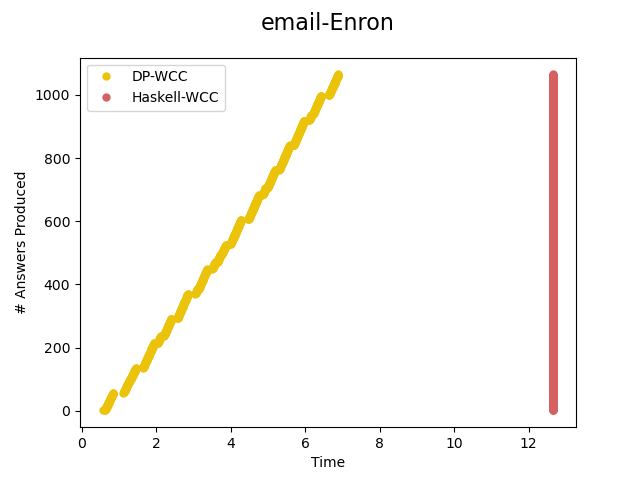
\includegraphics[width=1\linewidth, height=0.2\textheight]{email_enron}
      \caption[{[PoC] \acrshort{dm} Results: email-Enron}]{email-Enron \acrshort{dm}}
      \label{fig:dief:1}
    \end{subfigure}%
    \begin{subfigure}{0.33\textwidth}
     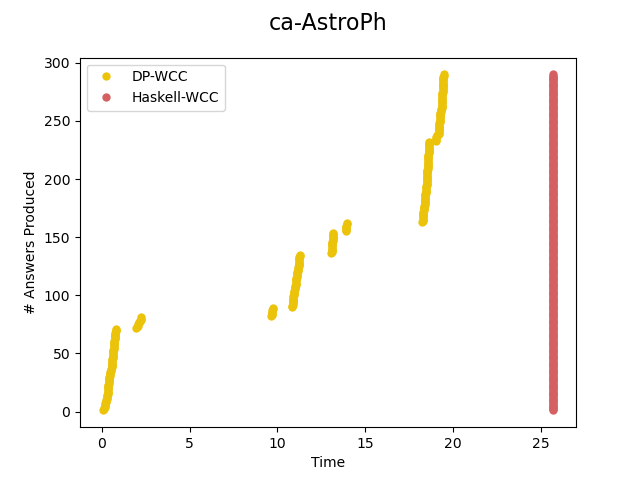
\includegraphics[width=1\linewidth, height=0.2\textheight]{ca_astroph}
      \caption[{[PoC] \acrshort{dm} Results: ca-AstroPh}]{ca-AstroPh \acrshort{dm}}
      \label{fig:dief:2}
    \end{subfigure}%
    \begin{subfigure}{0.33\textwidth}
     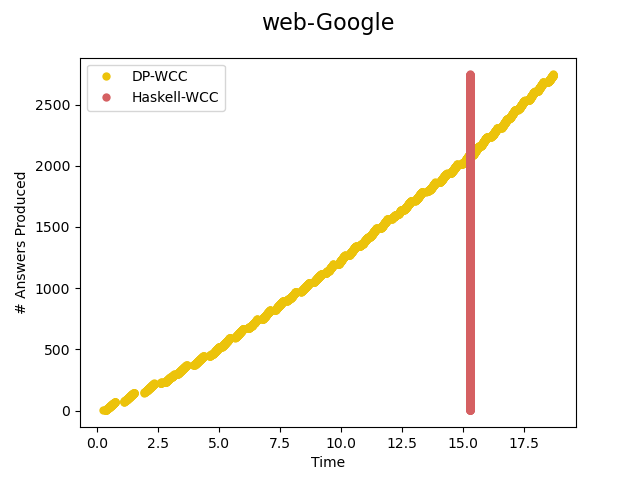
\includegraphics[width=1\linewidth, height=0.2\textheight]{web_google}
      \caption[{[PoC] \acrshort{dm} Results: web-Google}]{web-Google \acrshort{dm}}
      \label{fig:dief:3}
    \end{subfigure}
    \caption[{[PoC] \acrshort{dm} Metrics}]{This plots are showing the \acrshort{dm} on the three networks comparing both \acrshort{hs} implementations \acrshort{dpwcc} and \texttt{containers} lib. Red lines indicates \texttt{containers} \acrshort{hs} \acrshort{dm} metric. Yellow points indicates \acrshort{dpwcc} \acrshort{dm} metric}
\end{figure}

\begin{figure}[!htb]
  \centering
  \begin{subfigure}{0.33\textwidth}
   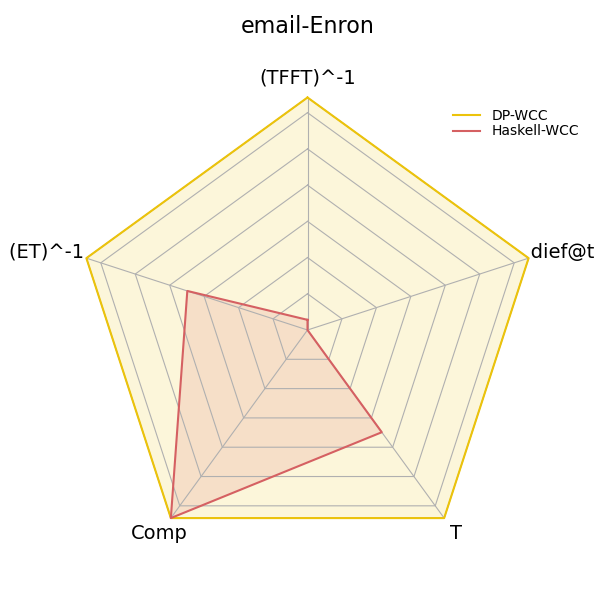
\includegraphics[width=1\linewidth, height=0.2\textheight]{email_enron_radar}
    \caption[{[PoC] \acrshort{dm} Results: email-Enron radar}]{email-Enron \acrshort{dm}}
    \label{fig:dief:rad:1}
  \end{subfigure}%
  \begin{subfigure}{0.33\textwidth}
   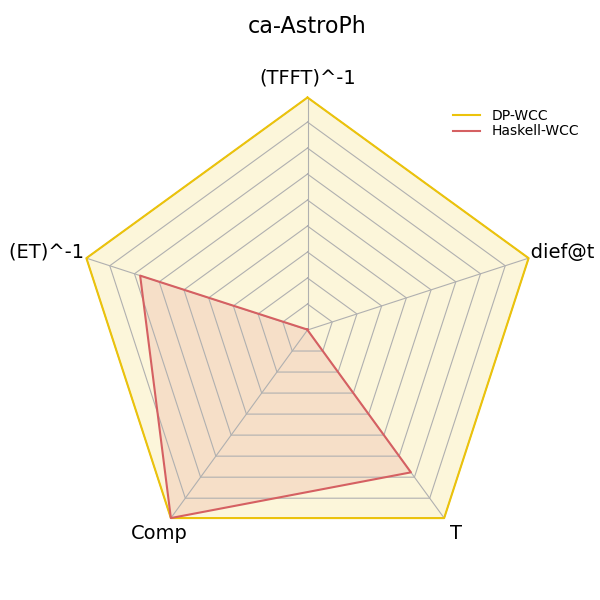
\includegraphics[width=1\linewidth, height=0.2\textheight]{ca_astroph_radar}
    \caption[{[PoC] \acrshort{dm} Results: ca-AstroPh radar}]{ca-AstroPh \acrshort{dm}}
    \label{fig:dief:rad:2}
  \end{subfigure}%
  \begin{subfigure}{0.33\textwidth}
   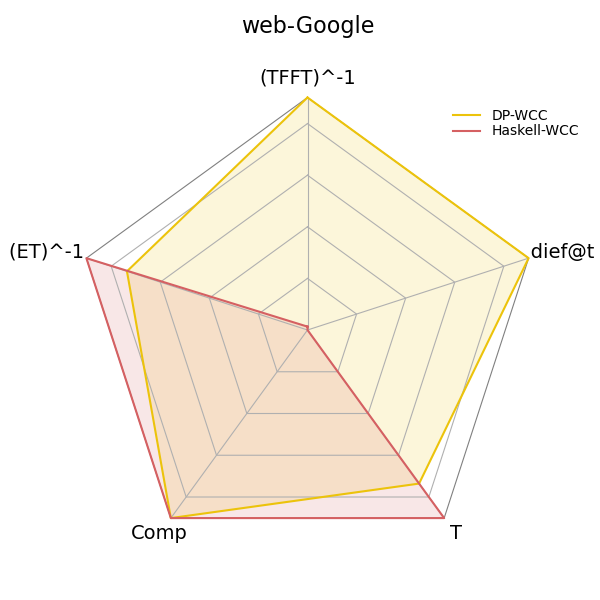
\includegraphics[width=1\linewidth, height=0.2\textheight]{web_google_radar}
    \caption[{[PoC] \acrshort{dm} Results: web-Google radar}]{web-Google \acrshort{dm}}
    \label{fig:dief:rad:3}
  \end{subfigure}
  \caption[{[PoC] \acrshort{dm} Metrics (Radial)}]{Radial plot shows how the different metrics provided by \acrshort{dm} tool such as \acrfull{tt}, \acrfull{tfft}, \acrfull{dt}, \acrfull{et} and \acrfull{comp} are related each other for each \acrshort{hs} implementation: \acrshort{dpwcc} and \texttt{containers}. Red area indicates \texttt{containers} \acrshort{hs} \acrshort{dm} metric. Yellow area indicates \acrshort{dpwcc} \acrshort{dm} metric}
\end{figure}

Based on the results shown in all the figures above, all the solutions in \acrshort{dpwcc} are being generated incrementally, 
but there is some difference that we would like to remark. In the case of \emph{email-Enron} and \emph{ca-AstroPh} graphs 
as we can see in \autoref{fig:dief:1} and \autoref{fig:dief:2}, there seems to be a more incremental generation of results. 
This behavior is measured with the values of \acrfull{dt}. \emph{ca-AstroPh} as it can be seen in \autoref{fig:dief:2}, is even more incremental, and it is showing a clear separation between some results and others. 
The \emph{web-Google} network, which is shown in \autoref{fig:dief:3}, is a little more linear, and that is because all the results are being generated with very little difference in time between them. 
Having the biggest \acrshort{wcc} at the end of \emph{web-Google} \acrshort{dp} algorithm 
it is retaining results until the biggest \acrshort{wcc} can be solved, which takes longer. 


\paragraph{Multithreading} For analyzing parallelization and multithreading we have used \textit{ThreadScope} \cite{threadscope} which allows us to see how the parallelization is taking place on \acrshort{ghc} at a fine grained level and how the threads are distributed throughout the different cores requested with the \mintinline{bash}{-N} execution \texttt{ghc-option} flag.
The distribution of the load is more intensive at the end of the execution, where \mintinline{haskell}{actor2} filter stage of the algorithm is taking place and different filters are reaching execution of that second actor.
We can appreciate how many threads are being spawned and by the tool and if they are evenly distributed among cores. 

\begin{figure}[!htb]
  \centering
  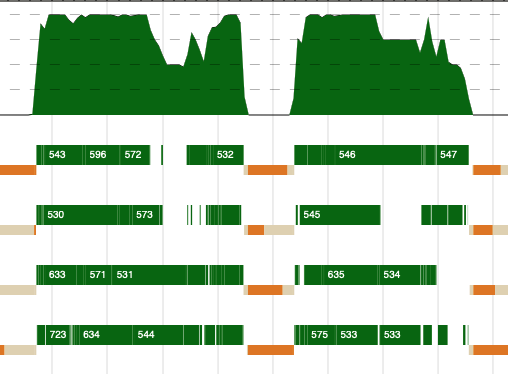
\includegraphics[width=0.7\textwidth, height=0.3\textheight]{screen_2}
  \caption[{[PoC] Thread Metrics: Fraction of Time}]{Threadscope Image of Zoomed Fraction of $10$ nanoseconds. Upper green area shows the amount of core used during that fraction of time. The lower are where it shows four separated green bars describe the behavior on each core. The number inside the green bar show the amount of threads running on that core at that moment. Finally orange bars are GC time.}
  \label{fig:4}
 \end{figure}

~\autoref{fig:4} zooms in on \textit{ThreadScope} output in a particular moment, approximately in the middle of the execution. 
The numbers inside green bars represent the number of threads that are being executed on that particular core (horizontal line) at that execution slot. 
Thus, the number of threads varies among slot execution times, because as it is already known, \acrshort{ghc} implements \emph{Preemptive Scheduling} \cite{lightweightghc}.
It can be appreciated in \autoref{fig:4} our first assumption that the load is evenly distributed because the mean number of executing threads per core is $571$.


\paragraph{Memory allocation} Another important aspect in our case is how the memory is being managed to avoid memory leaks or other non-desired behavior that increases memory allocation during the execution time. 
This is even more important in the particular implementation of \acrshort{wcc} using \acrshort{dp} model because it requires to maintain the set of connected components in memory throughout the execution of the program or at least until we can output the calculated \acrshort{wcc} if we reach to the last \textit{Filter} and we know that this \acrshort{wcc} cannot be enlarged anymore.
In order to verify this, we measure memory allocation with \textit{eventlog2html} \cite{eventlog2html} which converts generated profiling memory eventlog files into graphical HTML representation. 

\begin{figure}[!htb]
  \centering
  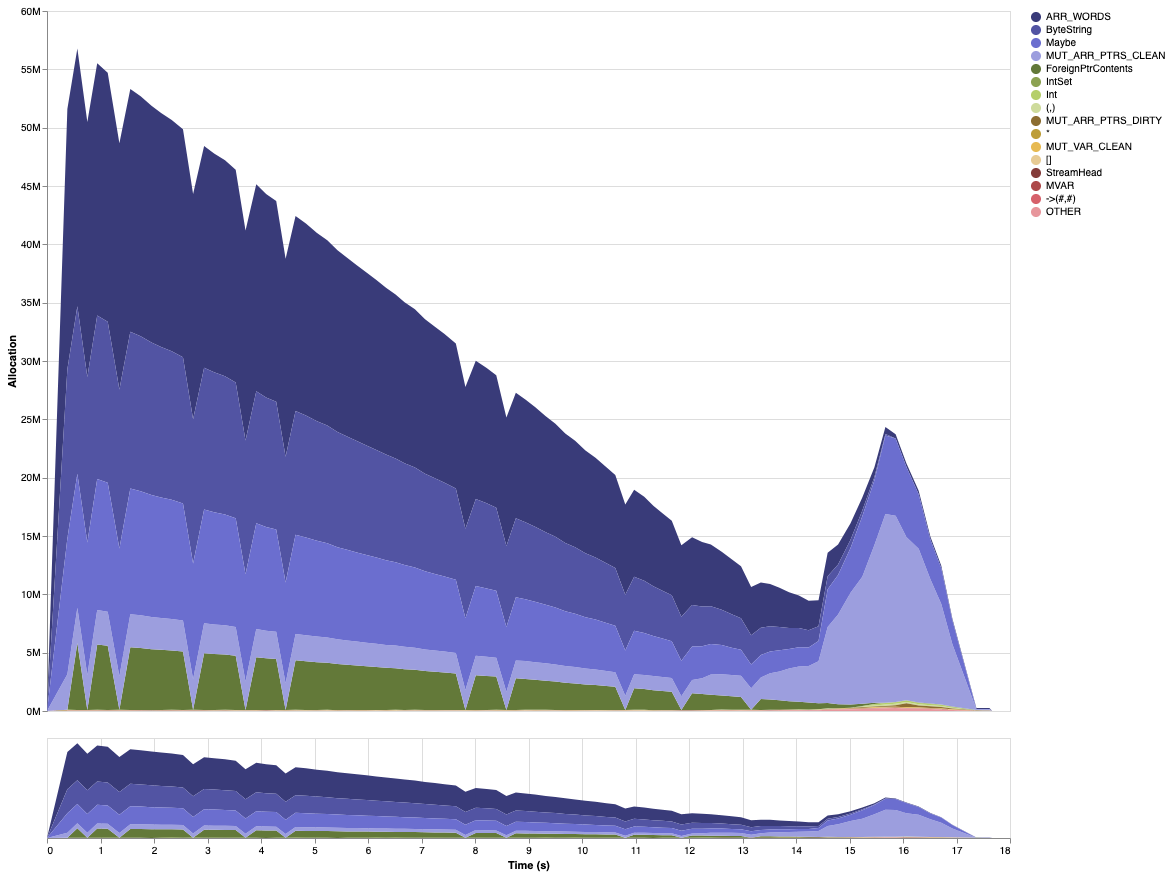
\includegraphics[width=1\linewidth, height=0.3\textheight]{visualization}
  \caption[{[PoC] Memory Metrics: Allocation by Data Type}]{This plot is showing the accumulated memory allocation size of each \acrshort{hs} Data Type throughout the execution of the program. The dark blue area shows the \texttt{ARR\_WORDS} data type which is \texttt{String} values. There are many of them because all that it comes from a file is in \texttt{String} format and need to be converted to the proper Data type. Rest of the light blue areas belong to \texttt{ByteString} which is the format treated in the input file as well, and \texttt{Maybe} type which is the type of data transfer between channels.}
  \label{fig:5}
\end{figure}

As we can see in \autoref{fig:5}, \acrshort{dpwcc} does efficient work on allocating memory since we are not using more than $57$ MB of memory during the whole execution of the program.
On the other hand, if we analyze how the memory is allocated during the execution of the program, it can also be appreciated that most of the memory is allocated at the beginning of the program and steadily decrease over time, with a small peak at the end that does not overpass even half of the initial peak of $57$ MB. 
The explanation for this behavior is quite straightforward because, in the beginning, we are reading from the file and transforming a \mintinline{haskell}{ByteString} buffer to \mintinline{haskell}{(Int, Int)} edges. 
This is seen in the image in which the dark blue that is on top of the area is \mintinline{haskell}{ByteString} allocation. 
Light blue is allocation of \mintinline{haskell}{Maybe a} type which is the type that is returned by the \textit{Channels} because it can contain a value or not. 
Data value \mintinline{haskell}{Nothing} is indicating end of the \textit{Channel}. 
Another important aspect is the green area which represents \mintinline{haskell}{IntSet} allocation, which in the case of our program is the data structure that we use to gather the set of vertices that represents a \acrshort{wcc}. 
This means that the amount of memory used for gathering the \acrshort{wcc} itself is minimum, and it is decreasing over time, which is another empirical indication that we are incrementally releasing results to the user. 
It can be seen as well that as long the green area reduces the lighter blue (\texttt{MUT\_ARR\_PTRS\_CLEAN} \cite{ghcheap}) increases at the same time indicating that the computations for the output (releasing results) is taking place. 
Finally, according to what we have stated above, we can answer the question [Q3], showing that not only the memory management was efficient, but at the same time, the memory was not leaking or increasing across the running execution program.

The empirical evaluation of the \acrshort{dpwcc} implementation to compute weakly connected components of a graph, evidence suitability, 
and robustness to provide a Dynamic Pipeline Framework in that language. Measuring using \par\bigskip metrics reveals some advantageous capability of $\dpwcc$ implementation to deliver incremental results compared with default containers library implementation. 
Regarding the main aspects where DPP is strong, i.e., pipeline parallelism and time processing, the $\dpwcc$ performance shows that Haskell 
can deal with the requirements for the \acrshort{wcc} problem without penalizing neither execution time nor memory allocation. 
In particular, the $\dpwcc$ implementation outperforms in those cases where the topology of the graph is sparse and where the number of vertices in the largest \acrshort{wcc} is not big enough. 
To conclude, the proof of concept has gathered enough evidence to show that the implementation of Dynamic Pipeline in Haskell Programming Language is feasible. 
This fact opens a wide range of algorithms to be explored using the Dynamic Pipeline Paradigm, supported by purely functional programming language.

\section{Chapter Summary}
In this chapter, we have presented a proof of concept that allows us to assess the feasibility of implementing \acrshort{dp} using \acrshort{hs}. 
The obtained results gave us insights about how to proceed for implementing a first version of a DPF using (parallel) Haskell and, afterward, to implement an algorithm for enumerating incrementally the bi-triangles of a bipartite graph based on the  \acrshort{dp}.


\chapter{Dynamic Pipeline Framework in Haskell}\label{dp-hs}
The design and implementation of \acrfull{dpfh} is a fundamental piece of the present work, as we have described in ~\autoref{intro} and ~\autoref{prelim},
A \acrlong{dpf} written in \acrlong{hs} which allow \acrshort{hs} users to implement any suitable algorithm in \acrlong{dp}.
During the process of conducting this research, we have implemented \acrshort{dpfh}~\cite{dynamic-pipeline} and publishes it into \acrlong{hack}~\cite{hackage}.
In this chapter, we describe the design and implementation details of \acrshort{dpfh}.

\section{Framework Design}

\subsection{Background}
Any suitable framework should provide the user the right level of abstraction that removes and hides underlying complexity, 
allowing the developer to focus on the problem that needs to be solved.
There are several design approximations to implement a framework: \begin{inparaenum}[i\upshape)]
  \item  \emph{Configuration Based} where the user only focuses on completing a specific configuration either on a file or a database or both. Once this configuration is completed, the user provides it to the framework's runtime system in order to execute the program. An example of this could be WordPress~\cite{wordpress},
  \item  \emph{Convention over Configuration (CoC)} where the user writes his code and definition following certain patterns in naming or source code location. With this source code and content-specific information, the framework interprets what is the execution flow that needs to be done on runtime. This technique have been deeply explored in the last $10$ years for different languages starting with Ruby on Rails~\cite{rubyonrails} which was the first on popularizing this design paradigm. Other examples are \cite{springboot, cakephp},
  \item \emph{Application Programing Interface (API)} where the framework or library provides a certain amount of functionality implemented in terms of functions or interfaces, and the user needs to compose those functions or implement those abstractions to achieve the desired results. This has been the traditional design paradigm for building any library or framework, and finally
  \item \emph{\acrfull{dsl}}~\cite{Fowler10} where the framework or library provides a new language that represents the domain problem that allows developing the solution in terms of that high-level language. An example of this type of design is Hibernate Query Language~\cite{hql}
   \end{inparaenum}.

There exists two types of \acrlong{dsl}s~\cite{dsl}: \acrlong{dsl} and \acrfull{edsl}. The purpose of \acrshort{dsl}, usually called external \acrshort{dsl}, is to create a completely new language with its own semantic, syntax, and interpreter. 
\acrshort{dsl}s are not general-purpose languages, because as their name indicates, they are domain-specific. \acrshort{edsl} are syntactically embedded in the host language of the library, and the user writes in that host language, but restricted by the \acrshort{edsl} abstractions.
\acrshort{dpfh} follows a \acrshort{edsl} approach taking advantage of the strong type \acrshort{hs} system giving the user correctness at type-level~\cite{curryhoward}.

\subsection{Architectural Design}
In this section we focus on the architectural design of the \acrshort{dpfh} using a \acrshort{edsl} approach. We have built a framework that contains
three important components: \acrshort{dsl}, \acrshort{idl} and \acrshort{rs}. 

\begin{figure}[!ht]
  \centering
   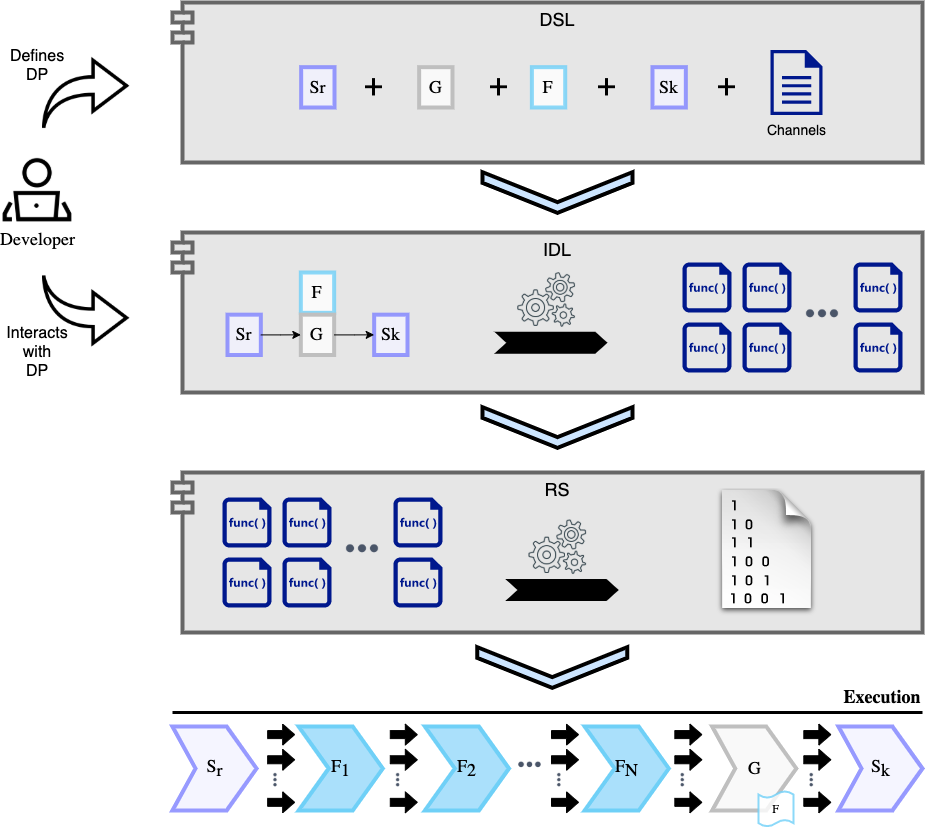
\includegraphics[width=1\textwidth, height=0.6\textheight]{dpf_haskell_v3.png}
    \caption[{[\acrshort{dpfh}] Architectural design of \acrshort{dpfh}}]{This diagram shows the architectural design of \acrshort{dpfh}. \acrshort{dpfh} is a \acrshort{dsl} which is built on three main components: \acrshort{dsl}, \acrshort{idl} and \acrshort{rs}. In the \acrshort{dsl} we can see how the user can compose the main stages of the \acrshort{dp}. \acrshort{idl} is showing how the frameworks is helping the user to transform that definition into real function or computations. Finally \acrshort{rs} execute all that definition plus functions. Execution layer indicates an example of a \acrshort{dp} running after being executed.}
    \label{fig:dpfh:1}
\end{figure}

In \autoref{fig:dpfh:1} we can appreciate the different components mentioned before that are the grey boxes.

\paragraph{DSL} The user interacts with the \acrshort{dsl} component where defines how the \acrshort{dp} flow
should be. Defining the flow consists on to provide a specification at type-level term about the channels that communicate each stage of the pipeline, as well as the data types those channels carry. 
For example, in the case of \autoref{prole} that we develop the \acrshort{wcc} algorithm, the user knows stages $\iwcc$, $\gwcc$, and $\owcc$ need to be connected with two channels. 
One of those channels is carrying the edges -- \texttt{Edge} data type -- and the other the accumulated connected components -- \texttt{ConnectedComp} data type --. 

\paragraph{IDL} Based on the definition provided in the \acrshort{dsl}, the user interacts with the \acrshort{idl} to build the functions with the algorithms needed for each stage: $\iwcc$, $\gwcc$, $\owcc$, $\fwcc$, and actors. 

\paragraph{RS} \acrshort{rs} is fed with the \acrshort{dp} definition and the functions implementations to finally execute the program. 

\section{Implementation}
In this section, we describe the details of all the techniques used for implementing each architectural layer described before.
As we have explained in \autoref{sec:contrib}, this library was published on Hackage~\cite{dynamic-pipeline}, the source code is open and can be found on this Github Repository~\cite{dynamic-pipeline-git}.

\subsection{DSL Grammar}\label{sub:sec:dsl-gram}
In order to provide a Type-safe verification in compilation time, we have defined a \acrfull{cfg} that generates a \acrshort{dp} \acrshort{dsl} language. 
\acrshort{cfg} enables the user to define a \acrshort{dp} at type-level. 

\begin{definition}[\acrshort{dsl} \acrshort{cfg}]\label{def:cfg:dsl}
Lets $\gdsl = (N, \Sigma, DB, P)$ be a Context-Free Grammar, such that $N$ is the set of non-terminal symbols, $\Sigma$ the set of terminal symbols,
$DP \in N$ is the start symbol and $P$ are the generation rules. \autoref{fig:def:dpfh:dsl} shows the formal definition of the grammar.
\begin{figure}[htp!]
\begin{equation*}
    \boxed{
      \begin{aligned}
    N &= \{DP,S_r,S_k,G,F_b,CH,CH_s\},\\
    \Sigma &= \{\text{\mintinline{haskell}{Source}},\text{\mintinline{haskell}{Generator}},\text{\mintinline{haskell}{Sink}},\text{\mintinline{haskell}{FeedbackChannel}},\text{\mintinline{haskell}{Type}},\text{\mintinline{haskell}{Eof}},\text{\mintinline{haskell}{:=>}},\text{\mintinline{haskell}{:<+>}}\},
    \end{aligned}
    }
\end{equation*}
\begin{equation*}
  \boxed{
    \begin{aligned}
  P = \{\\
  DP  &\rightarrow S_r\ \text{\mintinline{haskell}{:=>}}\ G\ \text{\mintinline{haskell}{:=>}}\ S_k\ |\ S_r\ \text{\mintinline{haskell}{:=>}}\ G\ \text{\mintinline{haskell}{:=>}}\ F_b\ \text{\mintinline{haskell}{:=>}}\ S_k,\\
  S_r &\rightarrow \text{\mintinline{haskell}{Source}}\ CH_s,\\
  G   &\rightarrow \text{\mintinline{haskell}{Generator}}\ CH_s,\\
  S_k &\rightarrow \text{\mintinline{haskell}{Sink}},\\
  F_b &\rightarrow \text{\mintinline{haskell}{FeedbackChannel}} CH,\\
  CH_s &\rightarrow \text{\mintinline{haskell}{Channel}}\ CH,\\
  CH &\rightarrow \text{\mintinline{haskell}{Type :<+>}}\ CH\ |\ \text{\mintinline{haskell}{Eof}}\}
\end{aligned}
}
\end{equation*}
\caption[{[\acrshort{dpfh}] DSL Grammar definition}]{This is the Context-Free Grammar defined for the DSL. In the first box we can see $N$ which is the set of non-terminals symbols of the Grammar. $\Sigma$ which is the set of the terminal symbols and $P$ the production rules of the grammar.}
\label{fig:def:dpfh:dsl}
\end{figure}
\end{definition}

In order to encode this on the language, we need an \emph{Index type}~\cite{type-index} to keep track of the information, at type-level, for generating the \acrshort{dp}. 
In that sense, we create an \emph{Index type} for each element of $\Sigma$.

\begin{listing}[htp!]
  \begin{minted}[fontsize=\small,numbers=left,breaklines,frame=lines,framerule=2pt,framesep=2mm,baselinestretch=1.2,highlightlines={3,4}]{haskell}

data Source (a :: Type)
data Generator (a :: Type)
data Sink
data Eof
data Channel (a :: Type)
data FeedbackChannel (a :: Type)

  \end{minted}
  \caption[{[\mintinline{shell}{Flow.hs}] $\Sigma$ enconding of $G_{dsl}$}]{This code is showing most of the data types that represent the same terminal symbols $\Sigma \in G_{dsl}$. Those types that are indexed by another kind \mintinline{haskell}{Type}, allows to store information at type-level needed for interpret the DSL}
  \label{src:dpfh:1}
\end{listing}
  
First, we can see in \autoref{src:dpfh:1}, some of the terminal symbols $\Sigma \in \gdsl$ encoded in \acrshort{hs} Types.
The highlighted lines in \autoref{src:dpfh:1} shows the only terminal symbols $\Sigma$ that are not indexed, because neither \mintinline{haskell}{Sink} nor \mintinline{haskell}{Eof} are carrying extra type-level information. 
In the case of \mintinline{haskell}{Sink}, since it is the last stage that does not connect further with any other stage, we do not need to indicate channel information. 
\mintinline{haskell}{Eof} it is just a terminal type to disambiguate the \mintinline{haskell}{Channel (a :: Type)} subtree for the full parser tree. 
\mintinline{haskell}{Channel} can carry any type because it needs to be polymorphic to support a different number of channels and data types.

\begin{listing}[htp!]
  \begin{minted}[fontsize=\small,numbers=left,breaklines,frame=lines,framerule=2pt,framesep=2mm,baselinestretch=1.2,highlightlines={1,5}]{haskell}
    
    data chann1 :<+> chann2 = chann1 :<+> chann2
    deriving (Typeable, Eq, Show, Functor, Traversable, Foldable, Bounded)
    infixr 5 :<+>
    
    data a :=> b = a :=> b
    deriving (Typeable, Eq, Show, Functor, Traversable, Foldable, Bounded)
    infixr 5 :=>
    
  \end{minted}
  \caption[{[\mintinline{shell}{Flow.hs}] $\Sigma$ enconding of $G_{dsl}$ - Especial non-terminals}]{Special terminal symbols $\{\text{\mintinline{haskell}{:<+>}}, \text{\mintinline{haskell}{:=>}}\} \in \Sigma$. This terminal symbols allows to index two types in order to combine several of them and build a chain of stages (\mintinline{haskell}{:=>}) and a set of channels (\mintinline{haskell}{:<+>}).}
  \label{src:dpfh:2}
\end{listing}

There are two more important terminal symbols in $\Sigma$: \mintinline{haskell}{:=>} and \mintinline{haskell}{:<+>}.
In \autoref{src:dpfh:2}, the definition shows how \mintinline{haskell}{:=>} and \mintinline{haskell}{:<+>} can combine 2 (two) types. 
The propose of writing \mintinline{haskell}{:=>} and \mintinline{haskell}{:<+>} as types is to have a syntactic sugar type combinator for writing the \acrshort{dsl} according to the \acrshort{cfg}. 
Apart from that, they are different because two distinguishable terminal symbols $\Sigma$ are needed to separate the encoding of the pipeline stage ($\iwcc$, $\gwcc$, $\owcc$)
from the encoding of channel composition in the same stage, as we can appreciate in \dref{def:cfg:dsl}.

Now, we can start defining our pipelines at type-level. For example, if we want to generate a \acrshort{dp} that eliminates duplicated elements in a stream, we know that we only need one channel connecting the stages that carries out the type of the element, in this case, \mintinline{haskell}{Int} (see \autoref{src:dpfh:3}).

\begin{listing}[htp!]
  \begin{minted}[fontsize=\small,numbers=left,breaklines,frame=lines,framerule=2pt,framesep=2mm,baselinestretch=1.2,highlightlines={}]{haskell}

type DPExample = Source (Channel (Int :<+> Eof)) 
              :=> Generator (Channel (Int :<+> Eof)) 
              :=> Sink
   
  \end{minted}
  \caption[{[\mintinline{shell}{Repeated.hs} Example of \acrshort{dp} encoded in $G_{dsl}$}]{This example shows the \acrshort{dsl} encoding in \acrshort{dp} of repeated elements problems}
  \label{src:dpfh:3}
\end{listing}

\subsection{DSL Validation}\label{sub:sec:dsl-val}
The language generated by the grammar needs to be validated to avoid errors or provide an incorrect \acrshort{dp} definition.
Fortunately, \acrshort{hs} provides several Type-level techniques~\cite{type-haskell} which allows to verify properties of programs before running them, 
preventing the users to introduce bugs, reducing errors. This verification done by the compiler establish a Curry-Howard Isomorphism~\cite{curryhoward}, i.e. 
\emph{Propositions as Types - Programs as Proof}. It is important to remark here that \acrshort{hs} is not a theorem prover System like Coq~\cite{coq}, but some verifications, as we present in this work, can be done with \acrshort{ghc} to ensure correctness on programs.
Although \acrshort{hs} provides tools to build advanced type-level verifications, all these techniques require the addition of \emph{Haskell Language Extensions}.

Once we have the encoded \acrshort{dp} problem in the \acrshort{dsl} grammar -- see \autoref{sub:sec:dsl-gram} --, we can proceed on validating that encoded grammar. 
The implementation of the validation of the \acrshort{dsl} \acrshort{cfg} at type-level, has been done using \emph{Associated Type Families}~\cite{associated-types}.

\begin{listing}[htp!]
  \begin{minted}[fontsize=\small,numbers=left,breaklines,frame=lines,framerule=2pt,framesep=2mm,baselinestretch=1.2,highlightlines={6,18}]{haskell}

type family And (a :: Bool) (b :: Bool) :: Bool where
    And 'True 'True = 'True
    And a b         = 'False
  

type family IsDP (dpDefinition :: k) :: Bool where
    IsDP (Source (Channel inToGen) :=> Generator (Channel genToOut) :=> Sink)
        = And (IsDP (Source (Channel inToGen))) (IsDP (Generator (Channel genToOut)))
    IsDP ( Source (Channel inToGen) :=> Generator (Channel genToOut) :=> FeedbackChannel toSource :=> Sink)
        = And (IsDP (Source (Channel inToGen))) (IsDP (Generator (Channel genToOut)))
    IsDP (Source (Channel (a :<+> more)))     
        = IsDP (Source (Channel more))
    IsDP (Source (Channel Eof))               = 'True
    IsDP (Generator (Channel (a :<+> more)))  = IsDP (Generator (Channel more))
    IsDP (Generator (Channel a))              = 'True
    IsDP x                                    = 'False
     
type family ValidDP (a :: Bool) :: Constraint where
  ValidDP 'True = ()
  ValidDP 'False = TypeError
                    ( 'Text "Invalid Semantic for Building DP Program"
                      ':$$: 'Text "Language Grammar:"
                      ':$$: 'Text "DP       -> Source CHANS :=> Generator CHANS :=> Sink"
                      ':$$: 'Text "DP       -> Source CHANS :=> Generator CHANS :=> FEEDBACK :=> Sink"
                      ':$$: 'Text "CHANS    -> Channel CH"
                      ':$$: 'Text "FEEDBACK -> FeedbackChannel CH"
                      ':$$: 'Text "CH       -> Type :<+> CH | Eof"
                      ':$$: 'Text "Example: 'Source (Channel (Int :<+> Int)) :=> Generator (Channel (Int :<+> Int)) :=> Sink'"
                    )
  \end{minted}
  \caption[{[\mintinline{shell}{Stage.hs}] Validating encoded in $G_{dsl}$ - FCF}]{Type Families \mintinline{haskell}{And}, \mintinline{haskell}{IsDP} and \mintinline{haskell}{ValidDP} which allows to perform a type-level validation over a \acrshort{dsl} \acrshort{cfg} definition.}
  \label{src:dpfh:4}
\end{listing}

In \autoref{src:dpfh:4}, there are 3(three) Type families that helps to validate the \acrshort{dsl} \acrshort{cfg}. 
\mintinline{haskell}{IsDP} associated type family is checking the production rules $P$ of the grammar defined in \autoref{fig:def:dpfh:dsl}, returning a promoted data type~\cite{promoted-types} (not a boolean value) \mintinline{haskell}{'True} in case
the production rule matches all the generated language, or \mintinline{haskell}{'False} otherwise. 
\mintinline{haskell}{ValidDP} is taking the result of \mintinline{haskell}{IsDP} type application, associating \mintinline{haskell}{'True} promoted boolean type to empty \mintinline{haskell}{()} constraint. An empty constraint is an 
indication of nothing to be restricted, meaning that if \mintinline{haskell}{ValidDP} is used as a constraint, and it is fully applied to \mintinline{haskell}{()}, it will give the compiler the evidence that there is no error at type-level.
\mintinline{haskell}{ValidDP} is also associating \mintinline{haskell}{'False} to a custom \mintinline{haskell}{TypeError} which will appear at compilation time if the \acrshort{dp} \acrshort{dsl} definition fully applies to that.

\begin{listing}[htp!]
  \begin{minted}[fontsize=\small,numbers=left,breaklines,frame=lines,framerule=2pt,framesep=2mm,baselinestretch=1.2,highlightlines={2}]{haskell}

mkDP :: forall dpDefinition filterState filterParam st.
    ( ValidDP (IsDP dpDefinition)
    , DPConstraint dpDefinition filterState st filterParam)
 => Stage (WithSource dpDefinition (DP st)) 
 -> GeneratorStage dpDefinition filterState filterParam st  
 -> Stage (WithSink dpDefinition (DP st))  
 -> DP st ()
mkDP = ...

someFunc = mkDP @DPExample ...

  \end{minted}
  \caption[{[\mintinline{shell}{Stage.hs}] Using validation of \acrshort{dp} encoded in $G_{dsl}$}]{Definition of \mintinline{haskell}{mkDP} function of the Framework which uses type-level validation of the grammar \mintinline{haskell}{ValidDP (IsValid Type)}. Last line of the code is showing that using that function will compile-time check the definition of \mintinline{haskell}{DPExample} type.}
  \label{src:dpfh:5}
\end{listing}

\subsection{\acrfull{idl}}
\acrshort{idl} component takes the \acrshort{dp} definition made on with \acrshort{dsl} component to interpret and generate the function definitions
that the user needs to fill in for solving a specific problem. In \autoref{sec:dp}, we have described what the user needs to provide in a \acrshort{dp} algorithm: $\iwcc$, $\gwcc$, $\owcc$, and the $\fwcc$ with the non-empty set of Actors.
The \acrshort{idl} generates the function definitions with an empty implementation to be completed by the user, ensuring that those functions will give "Proof" -- in terms of Curry-Howard Correspondence~\cite{curryhoward} --  of the "Propositions" defined on the \acrshort{dsl}.

Similar techniques that we used on \autoref{sub:sec:dsl-val} are also used here. 
On the first hand, \emph{Type-level Defunctionalization}~\cite{defunctionalization, fun-type-function-haskell} technique to let the compiler generates the signatures of the required functions. 
On the other hand, \emph{Term-level Defunctionalization} to interpret those functions.
Moreover, \emph{Indexed Types}~\cite{type-index} and \emph{Heterogeneous List}~\cite{hlist} are used to keep track of the dynamic number and polymorphic types of the functions parameters. 

\begin{listing}[htp!]
  \begin{minted}[fontsize=\small,numbers=left,breaklines,frame=lines,framerule=2pt,framesep=2mm,baselinestretch=1.2,highlightlines={2,6,10}]{haskell}

withSource :: forall (dpDefinition :: Type) st. WithSource dpDefinition (DP st) 
            -> Stage (WithSource dpDefinition (DP st))
withSource = mkStage' @(WithSource dpDefinition (DP st))

withGenerator :: forall (dpDefinition :: Type) (filter :: Type) st. WithGenerator dpDefinition filter (DP st) 
              -> Stage (WithGenerator dpDefinition filter (DP st))
withGenerator = mkStage' @(WithGenerator dpDefinition filter (DP st))

withSink :: forall (dpDefinition :: Type) st. WithSink dpDefinition (DP st) 
           -> Stage (WithSink dpDefinition (DP st))
withSink = mkStage' @(WithSink dpDefinition (DP st))
  \end{minted}
  \caption[{[\mintinline{shell}{Stage.hs}] Using with Interpreters of \acrshort{dp} encoded in $G_{dsl}$}]{This code is showing the different interpreters combinators to help the user to generate the functions of the principal stages of \acrshort{dp}}
  \label{src:dpfh:6}
\end{listing}

In \autoref{src:dpfh:6} we can appreciate the different combinators of the \acrshort{idl} that helps the user of the framework to interpret the \acrshort{dsl} to generate the function definitions.
\mintinline{haskell}{Stage} data type will be cover in \autoref{src:dpfh:8}, but it is a wrapper type of a pipeline stage -- minimal unit of execution --, containing the function to be executed -- here is the use \emph{Term-level Defunctionalization} --.
\mintinline{haskell}{withSource}, \mintinline{haskell}{withGenerator}, and \mintinline{haskell}{withSink} are syntactic sugar of the function \mintinline{haskell}{mkStage'} which is the combinator that is applying the \emph{Associated Type} related to that stage. For example \mintinline{haskell}{withSource}, is equivalent to \mintinline{haskell}{mkStage' @(WithSource dpDefinition (DP st))}.
For each \emph{Associated Type Family} defintion, there exist an equivalent term-level definition: \mintinline{haskell}{WithSource} type with \mintinline{haskell}{withSource} term , \mintinline{haskell}{WithGenerator} type with \mintinline{haskell}{withGenerator} term, and \mintinline{haskell}{WithSink} type with \mintinline{haskell}{withSink} term -- notice the capital case letter "W" indicating the type and not the term --.

\begin{listing}[htp!]
  \begin{minted}[fontsize=\small,numbers=left,breaklines,frame=lines,framerule=2pt,framesep=2mm,baselinestretch=1.2,highlightlines={7,11}]{haskell}

type family WithSource (dpDefinition :: Type) (monadicAction :: Type -> Type) :: Type where
  WithSource (Source (Channel inToGen) :=> Generator (Channel genToOut) :=> Sink) monadicAction
      = WithSource (ChanIn inToGen) monadicAction
  WithSource (Source (Channel inToGen) :=> Generator (Channel genToOut) :=> FeedbackChannel toSource :=> Sink) monadicAction 
      = WithSource (ChanOutIn toSource inToGen) monadicAction
  WithSource (ChanIn (dpDefinition :<+> more)) monadicAction         
      = WriteChannel dpDefinition -> WithSource (ChanIn more) monadicAction
  WithSource (ChanIn Eof) monadicAction                              
      = monadicAction ()
  WithSource (ChanOutIn (dpDefinition :<+> more) ins) monadicAction  
      = ReadChannel dpDefinition -> WithSource (ChanOutIn more ins) monadicAction
  WithSource (ChanOutIn Eof ins) monadicAction                       
      = WithSource (ChanIn ins) monadicAction
  WithSource dpDefinition _                                          
      = TypeError
          ( 'Text "Invalid Semantic for Source Stage"
            ':$$: 'Text "in the DP Definition '"
            ':<>: 'ShowType dpDefinition
            ':<>: 'Text "'"
            ':$$: 'Text "Language Grammar:"
            ':$$: 'Text "DP       -> Source CHANS :=> Generator CHANS :=> Sink"
            ':$$: 'Text "DP       -> Source CHANS :=> Generator CHANS :=> FEEDBACK :=> Sink"
            ':$$: 'Text "CHANS    -> Channel CH"
            ':$$: 'Text "FEEDBACK -> FeedbackChannel CH"
            ':$$: 'Text "CH       -> Type :<+> CH | Eof"
            ':$$: 'Text "Example: 'Source (Channel (Int :<+> Int)) :=> Generator (Channel (Int :<+> Int)) :=> Sink'"
          )
  \end{minted}
  \caption[{[\mintinline{shell}{Stage.hs}] WithSource Associate Type Details}]{An example of the Associated Type Family \mintinline{haskell}{WithSource} that allows to implement \emph{Type-level Defunctionalization} technique that will be the Type-level verification of the term \mintinline{haskell}{withSource}}
  \label{src:dpfh:7}
\end{listing}

In \autoref{src:dpfh:7}, in the highlighted lines, it can be seen how \emph{Type-level Defunctionalization} is being expanded in a signature function definition of the form \mintinline{haskell}{a -> b -> ...} depending on \acrshort{dp} language definition. 

\begin{listing}[htp!]
  \begin{minted}[fontsize=\small,numbers=left,breaklines,frame=lines,framerule=2pt,framesep=2mm,baselinestretch=1.2,highlightlines={12,16}]{haskell}

data Stage a where
  Stage :: Proxy a -> a -> Stage a

mkStage' :: forall a. a -> Stage a
mkStage' = Stage (Proxy @a)
    
  \end{minted}
  \caption[{[\mintinline{shell}{Stage.hs}] Stage Data Type}]{\mintinline{haskell}{Stage} data type for implementing \emph{Term-level Defunctionalization} providing evidence to the Type-Level Associated types}
  \label{src:dpfh:8}
\end{listing}

In \autoref{src:dpfh:8}, \mintinline{haskell}{Stage} data type uses a \mintinline{haskell}{Proxy a} phantom type. 
This phantom type allow \mintinline{haskell}{Stage} to index the type definition generated by \mintinline{haskell}{a}.
For example, in \autoref{src:dpfh:6}, \mintinline{haskell}{withSource} interpreter is applied to \mintinline{haskell}{WithSource dpDefinition}. 
Therefore when the compiler is provided with \mintinline{haskell}{dpDefinition} \acrshort{dsl} type, it expands the function signature belonging to that \acrshort{dp} definition inside the \mintinline{haskell}{Stage}.

\paragraph{Generator and Filter}
Generator ($\gwcc$) and Filter ($\fwcc$) should be explained together because as we have seen on \acrshort{dp} definition in \autoref{sec:dp},
$\gwcc$ has a $\fwcc$ template in order to know how to dynamically interpose a new $\fwcc$ during the runtime execution of the program.
Let's first study $\fwcc$ Data Type in the context of the framework.

\begin{listing}[htp!]
  \begin{minted}[fontsize=\small,numbers=left,breaklines,frame=lines,framerule=2pt,framesep=2mm,baselinestretch=1.2,highlightlines={2,5}]{haskell}

newtype Actor dpDefinition filterState filterParam monadicAction =
    Actor {  unActor :: MonadState filterState monadicAction => Stage (WithFilter dpDefinition filterParam monadicAction) }

newtype Filter dpDefinition filterState filterParam st =
    Filter { unFilter :: NonEmpty (Actor dpDefinition filterState filterParam (StateT filterState (DP st))) }
    deriving Generic
    
  \end{minted}
  \caption[{[\mintinline{shell}{Stage.hs}] Filter / Actor Data Type}]{This code shows the definition of the \mintinline{haskell}{Filter} data type which contains a non-empty set of \mintinline{haskell}{Actor}. The \mintinline{haskell}{Actor} data type is an \mintinline{haskell}{Stage} in the Context of the \mintinline{haskell}{MonadState} to allow keeping a local memory in the execution context of the filter.}
  \label{src:dpfh:9}
\end{listing}

In \autoref{src:dpfh:9} the definition of the \mintinline{haskell}{Filter} data type contains a non-empty set of \mintinline{haskell}{Actor}.
An \mintinline{haskell}{Actor} is a \mintinline{haskell}{Stage}, because by \acrshort{dp} definition in \autoref{sec:dp}, an actor is the minimal unit of execution of a filter. 
A \mintinline{haskell}{Filter} is a \mintinline{haskell}{NonEmpty Actor} -- Non-empty List -- because also by definition of \acrshort{dp} a filter is built by a sequence of actors calls. 
Moreover, \mintinline{haskell}{Actor} Stage is defunctionalized with \mintinline{haskell}{WithFilter} \emph{Associated Type Family} with the same concept as we have explained before for the other stages. 
\mintinline{haskell}{Filter} runs in an explicit \mintinline{haskell}{StateT} monadic context. This is because the $\fwcc$ instance should have an state, by \acrshort{dp} definition in \autoref{sec:dp}.
For example, in the case of $\dpwcc$, as we have seen in \autoref{prole} $\fwcc$ keeps an updated list of connected components that updates as long as it receives more edges that are connected with the current list.
\mintinline{haskell}{Actor} data type, in \autoref{src:dpfh:9}, is constrained by \mintinline{haskell}{MonadState} which is in the same execution context of the whole \mintinline{haskell}{NonEmpty Actor} list of the \mintinline{haskell}{Filter}. 
This means the \mintinline{haskell}{StateT} is executed for each \mintinline{haskell}{Actor} of that filter, sharing the same state between them. 

\begin{listing}[htp!]
  \begin{minted}[fontsize=\small,numbers=left,breaklines,frame=lines,framerule=2pt,framesep=2mm,baselinestretch=1.2,highlightlines={}]{haskell}

mkFilter :: forall dpDefinition filterState filterParam st. WithFilter dpDefinition filterParam (StateT filterState (DP st)) 
         -> Filter dpDefinition filterState filterParam st
mkFilter = Filter . single

single :: forall dpDefinition filterState filterParam st. WithFilter dpDefinition filterParam (StateT filterState (DP st)) 
       -> NonEmpty (Actor dpDefinition filterState filterParam (StateT filterState (DP st)))
single = one . actor

actor :: forall dpDefinition filterState filterParam st. WithFilter dpDefinition filterParam (StateT filterState (DP st)) 
      -> Actor dpDefinition filterState filterParam (StateT filterState (DP st))
actor = Actor . mkStage' @(WithFilter dpDefinition filterParam (StateT filterState (DP st)))

(|>>>) :: forall dpDefinition filterState filterParam st. Actor dpDefinition filterState filterParam (StateT filterState (DP st)) 
       -> Filter dpDefinition filterState filterParam st 
       -> Filter dpDefinition filterState filterParam st
(|>>>) a f = f & _Wrapped' %~ (a <|)
infixr 5 |>>>

(|>>) :: forall dpDefinition filterState filterParam st. Actor dpDefinition filterState filterParam (StateT filterState (DP st)) 
      -> Actor dpDefinition filterState filterParam (StateT filterState (DP st)) 
      -> Filter dpDefinition filterState filterParam st
(|>>) a1 a2 = Filter (a1 <|one a2)
infixr 5 |>>
  \end{minted}
  \caption[{[\mintinline{shell}{Stage.hs}] Filter / Actor smart constructors and combinators}]{Combinators and small constructor to enable building actors and filter.}
  \label{src:dpfh:10}
\end{listing}

Finally, in \autoref{src:dpfh:10}, some combinators and smart constructors are provided in the framework to enable the construction of \mintinline{haskell}{Filter} and \mintinline{haskell}{Actor}.
\mintinline{haskell}{mkFilter} is a smart constructor for \mintinline{haskell}{Filter} Data Constructor. \mintinline{haskell}{single} wraps one actor inside a \mintinline{haskell}{Filter}.
\mintinline{haskell}{actor} is a smart constructor for \mintinline{haskell}{Actor} Data Constructor. \mintinline{haskell}{(|>>>)} is an appending combinator of an \mintinline{haskell}{Actor} to a \mintinline{haskell}{Filter}. 
\mintinline{haskell}{(|>>>)} also ensures actor execution order, i.e. the latest actor added is the latest to be executed.


\begin{listing}[htp!]
  \begin{minted}[fontsize=\small,numbers=left,breaklines,frame=lines,framerule=2pt,framesep=2mm,baselinestretch=1.2,highlightlines={}]{haskell}
    data GeneratorStage dpDefinition filterState filterParam st = GeneratorStage
    { _gsGenerator      :: Stage (WithGenerator dpDefinition (Filter dpDefinition filterState filterParam st) (DP st))
    , _gsFilterTemplate :: Filter dpDefinition filterState filterParam st
    }  
  \end{minted}
  \caption[{[\mintinline{shell}{Stage.hs}] Generator}]{\mintinline{haskell}{Generator} Data type which contains the \mintinline{haskell}{Stage} code of the generator itself, and the \mintinline{haskell}{Filter} template that it can be spawned by the \mintinline{haskell}{Generator}.}
  \label{src:dpfh:11}
\end{listing}

In \autoref{src:dpfh:11}, $\gwcc$ contains a $\fwcc$ template and its own stage behavior.
\mintinline{haskell}{Generator} data type has a field with the \mintinline{haskell}{Filter} template that could be spawned by the algorithm defined by the user according to the data received from its input channels.
\mintinline{haskell}{Generator} has also another field with the behavior of the $\gwcc$ -- a \mintinline{haskell}{Stage} --. 

\subsection{\acrfull{rs}}
The \acrshort{rs} can be divided into two parts: the combinators generate stages dynamically in runtime, as long as data arrives at $\gwcc$,
and the execution context of the \acrshort{dp}.
Regarding execution context, all the stages that we have seen in previous sections are the pieces needed to build an executable \mintinline{haskell}{DP st a} monad.
This executable monad has an existential type similar to \mintinline{haskell}{ST} monad to not escape out from the context on different stages.
Once the dynamic pipeline starts to execute, the core of the framework dynamically generates stages between $\gwcc$ and previous stages, according to the user definition. 
This is an \emph{anamorphism}~\cite{lenses} that creates $\fwcc$ instances until some condition is met.

\begin{listing}[htp!]
  \begin{minted}[fontsize=\small,numbers=left,breaklines,frame=lines,framerule=2pt,framesep=2mm,baselinestretch=1.2,highlightlines={2,12,14,15,16,17,18}]{haskell}
unfoldF :: forall dpDefinition readElem st filterState filterParam l. SpawnFilterConstraint dpDefinition readElem st filterState filterParam l
        => UnFoldFilter dpDefinition readElem st filterState filterParam l 
        -> DP st (HList l) 
unfoldF = loopSpawn

where
  loopSpawn uf@UnFoldFilter{..} =
    maybe (pure _ufRsChannels) (loopSpawn <=< doOnElem uf) =<< DP (pull _ufReadChannel)

  doOnElem uf@UnFoldFilter{..} elem' = do
    _ufOnElem elem'
    if _ufSpawnIf elem'
     then do
       (reads', writes' :: HList l3) <- getFilterChannels <$> DP (makeChansF @(ChansFilter dpDefinition))
       let hlist = elem' .*. _ufReadChannel .*. (_ufRsChannels `hAppendList` writes')
       void $ runFilter _ufFilter (_ufInitState elem') hlist (_ufReadChannel .*. (_ufRsChannels `hAppendList` writes'))
       return $ uf { _ufReadChannel = hHead reads', _ufRsChannels = hTail reads' }
     else return uf

  \end{minted}
  \caption[{[\mintinline{shell}{Stage.hs}] unfoldF}]{\mintinline{haskell}{unfolF} is the \emph{anamorphism} combinator to spawn new \mintinline{haskell}{Filter} types between the \mintinline{haskell}{Generator} and previous stages.}
  \label{src:dpfh:12}
\end{listing}

In \autoref{src:dpfh:12} the \mintinline{haskell}{unfoldF} receives an \mintinline{haskell}{UnFoldFilter} Data type, which contains the recipe for controlling that unfold recursive call. 
In line 12, \mintinline{haskell}{_ufSpawnIf} field of \mintinline{haskell}{UnFoldFilter}, indicates when to stop the recursion. 
Inside the conditional, in the first line, we create new channels for that filter because we need to connect this new filter computation with the previous and with \mintinline{haskell}{Generator}. 
Therefore, the next stage is fed with the new channels of this new filter. After that, we call \mintinline{haskell}{runFilter} in line $16$, to put the computation 
to work in the pipeline -- call to \mintinline{haskell}{async} with \mintinline{haskell}{runStateT} --. Finally, we return the new channels to the $\gwcc$.
\mintinline{haskell}{HList}~\cite{hlist} is used for handling the dynamic number and parameters types of the generated functions.

\begin{listing}[htp!]
  \begin{minted}[fontsize=\small,numbers=left,breaklines,frame=lines,framerule=2pt,framesep=2mm,baselinestretch=1.2,highlightlines={}]{haskell}
mkUnfoldFilter :: (readElem -> Bool) 
    -> (readElem -> DP st ()) 
    -> Filter dpDefinition filterState filterParam st 
    -> (readElem -> filterState)
    -> ReadChannel readElem
    -> HList l 
    -> UnFoldFilter dpDefinition readElem st filterState filterParam l


mkUnfoldFilterForAll' :: (readElem -> DP st ())
                      -> Filter dpDefinition filterState filterParam st
                      -> (readElem -> filterState)
                      -> ReadChannel readElem
                      -> HList l
                      -> UnFoldFilter dpDefinition readElem st filterState filterParam l

mkUnfoldFilterForAll :: Filter dpDefinition filterState filterParam st
                      -> (readElem -> filterState)
                      -> ReadChannel readElem
                      -> HList l
                      -> UnFoldFilter dpDefinition readElem st filterState filterParam l
   \end{minted}
  \caption[{[\mintinline{shell}{Stage.hs}] UnfoldFilter combinators}]{Combinators for building \mintinline{haskell}{UnfoldFilter} types indicating the type of the \mintinline{haskell}{unfold} that the user want to achieve.}
  \label{src:dpfh:13}
\end{listing}

Several smart constructors are also provided for building \mintinline{haskell}{UnfoldFilter} Data Type.
In \autoref{src:dpfh:13} the first combinator is the default smart constructor. First parameter \mintinline{haskell}{(readElem -> Bool)} indicate if the a new filter should 
be spawn or not, allowing the user to inspect the each element of the incomming channel to take that decision. Second parameter \mintinline{haskell}{(readElem -> DP st ())} is a monadic optional computation to do when received a new element, for example logging.
Next to that is the \mintinline{haskell}{Filter} data type which is what is spawned. Continuing to that, \mintinline{haskell}{(readElem -> filterState)} is initialization of the \mintinline{haskell}{Filter} State. 
It also allows the user to initialize the state based on the first element received. 
Each filter is fed by a \mintinline{haskell}{(ReadChannel readElem)}. Finally, the last parameter is the \emph{Heterogeneous List} with the rest of the channels to connect with other stages.
The combinator \mintinline{haskell}{mkUnfoldFilterForAll} is to indicate to the framework that for each element received in the $\gwcc$, a new filter should be spawn.

\section{Libraries and Tools}
\subsection{Parallelization} 
One of the most important components of the implementation is the selection of concurrency libraries to support an intensive parallelization workload. Parallelization techniques and tools have been intensively studied and implemented in \acrshort{hs} \cite{monadpar}. 
Indeed, it is well known that green threads and sparks allow spawning thousands to millions of parallel computations. 
These parallel computations do not penalize performance when compare with \acrfull{os} level threading \cite{parallelbook}. 
A straightforward assumption to achieve here, is to use \texttt{monad-par} library \cite{monadparlib, monadpar}. 
Nevertheless, in this work, we have discarded the use of sparks \cite{sparks} because we can achieve the level of required parallelism spawning green threads only.
The next obvious choice is to use \mintinline{haskell}{forkIO :: IO () -> IO ThreadId} from \texttt{base} library \cite{forkio}. 
However, that would imply handling all the threads lifecycles and errors programmatically without any abstraction to facilitate that complex task. 
Therefore, we choose \texttt{async} library \cite{async} which enables to spawn asynchronous computations \cite{parallelbook} on \acrshort{hs} using green threads, and at the same time, it provides useful combinators to managing thread terminations and errors.

\subsection{Channels\label{section:channels}} 
We have several techniques to our disposal to communicate between threads or sparks in \acrshort{hs} like \mintinline{haskell}{MVar} or concurrent safe mechanisms like \acrfull{stm} \cite{stm}. 
At the same time, in \acrshort{hs} library ecosystem, we dispose of \texttt{Channels} abstractions based on both mentioned communication techniques. 
In that sense, for conducting the communication between dynamic stages and data flowing in a \acrshort{dp}, we have selected \texttt{unagi-chan} library \cite{unagi} which provides the following advantages to our solution: Firstly, \mintinline{haskell}{MVar} channel without using \acrshort{stm} reducing overhead. 
\acrshort{stm} is not required in a \acrshort{dp} because one specific stage which is running in a separated thread, can only access to its \texttt{I/O} channels for reading/writing accordingly, and those operations are not concurrently shared by other threads (stages) for the same channels. 
Second, non-blocking channels. \texttt{unagi-chan} library contains blocking and non-blocking channels for reading. This aspect is key to gain speed up on the implementation. Third, the library is optimized for $x86$ architectures with use of low-level \texttt{fetch-and-add} instructions. Finally, \texttt{unagi-chan} is $100x$ faster~\cite{unagi-bench} on Benchmarking compare with \acrshort{stm} and default base \mintinline{haskell}{Chan} implementations.

\section{Chapter Summary}
In this chapter, we have described with a great level of detail how \acrlong{dpfh} has been conceived from a Design point of view, 
as well as all the \acrshort{hs} data types and language techniques that we use for that implementation. 
At the end of the chapter, we have mentioned external libraries used for the runtime system and the reason for their choice.


\bibliographystyle{alpha}
\bibliography{Report}

\appendix

\end{document}

